\documentclass[10pt,letterpaper]{article}
\usepackage[margin=1in]{geometry}
\usepackage{amsmath}
\usepackage{amssymb}
\usepackage{graphicx}
\usepackage{cite}
\usepackage{booktabs}
\usepackage{float}
\usepackage{tabularx}
\usepackage{hyperref}
\usepackage{caption}
\usepackage{subcaption}
\usepackage{longtable}
\usepackage{float}
\setlength{\parindent}{0pt}
\setlength{\parskip}{0.5em}

\title{Estimating the Causal Effect of Extracurricular Activities on Student Performance}
\author{Yijiao Zhou\\ \texttt{yijiao\_zhou@berkeley.edu}}

\date{}


\begin{document}

\maketitle

% \begin{abstract}

% This project investigates the causal relationship between extracurricular activity participation and student exam scores using observational data. We start with ordinay least squares (OLS) regression to estimate the average treatment effect (ATE) while controlling for observed covariates. We then explore potential treatment effect heterogeneity by including interaction terms between the treatment and selected covariates. Finally, we implement inverse probability weighting (IPW) based on propensity scores to further adjust for confounding bias. The results consistently indicate a positive association between extracurricular activities and exam scores, with estimated effects around 0.5 to 0.6 points higher for participants compared to non-participants. However, the magnitude of the estimated effect is sensitive to influential observations, although the overall conclusion of a positive effect remains robust. The exploration of treatment effect heterogeneity did not yield statistically significant interaction effects, suggesting that the benefit of extracurricular activities on exam scores does not vary strongly across different levels of motivation or study hours in this dataset. The propensity score diagnostics indicate that the IPW approach successfully balanced the covariates between treatment groups, lending credibility to the causal interpretation of the estimated effects under the unconfoundedness assumption.
% \end{abstract}

\section{Introduction}

Understanding the factors that influence student performance is crucial for educators, policymakers, and students themselves. Extra-curricular activity has been widely debated in terms of its impact on academic performance. Some argue that it enhances time management and social skills, while others suggest it may detract from study time. The primary goal of this project is to estimate the causal effect of extra-curricular activities on student exam scores, while controlling for other factors that may influence both the likelihood of participating in extra-curricular activities and academic performance.

\section{Data}

Our data come from Kaggle's \href{https://www.kaggle.com/datasets/grandmaster07/student-exam-performance-dataset-analysis/data}{ ``Student Exam Performance Dataset Analysis''} \cite{kaggle_student_performance}, which contains information on students's academic, lifestyle and socioeconomic factors. After data cleaning and preprocessing, we have 6,378 complete cases for analysis. Basic data summary is provided in the Appendix~\ref{sec:data summary}.

For our problem, we are particularly interested in two key variables: Extracurricular Activities (the treatment variable) and Exam Score (the outcome variable). For naîve comparison, the mean difference in exam scores between students who participate in extracurricular activities and those who do not is around 0.503, which leads to a natural guess that students who participate in extracurricular activities tend to have slightly higher exam scores on average. 

In order to find the potential confounding factors, we use SMD (standardized mean difference) to compare the covariate distributions between the treatment and control groups. Figure~\ref{fig:smd_all} in Appendix~\ref{sec: smd} shows the largest SMD is around 0.06, which suggests that the covariates are reasonably balanced between the treatment and control groups. We choose to keep all the covariates in the model to control for potential confounding bias, as they are all theoretically relevant to the relationship between extracurricular activities and exam scores.

\section{Main Regression Model}

\subsection{Causal Inference Assumptions}

Because the data are observational rather than experimental, identification of the causal effect of extracurricular activities on exam scores relies on several standard assumptions \cite{ding_first_2023}.

\begin{itemize}
    \item \textbf{Unconfoundedness}: Conditional on the observed covariates $X$, treatment assignment is independent of the potential outcomes:
    \[
    Y(0), Y(1) \perp T \mid X.
    \]

    \item \textbf{Overlap (Positivity)}: Each student has a positive probability of receiving either treatment level:
    \[
    0 < P(T=1 \mid X) < 1.
    \]

    \item \textbf{SUTVA}: One student’s potential outcomes are unaffected by the treatment assignments of other students, and the treatment is consistently defined across units.
\end{itemize}




\subsection{Model Specification}

Under the assumptions above and the linear model is correctly specified, the average treatment effect (ATE) can be estimated using ordinary least squares (OLS). The model is specified as:

\begin{equation*}
Y_i = \alpha_0 + \alpha_1 T_i + X_i^T \alpha + \epsilon_i
\end{equation*}

where $\alpha_1$ represents the main effect of extracurricular activities on exam scores, conditional on covariates $X_i$.

\subsection{Results}
\subsubsection{Main Effect Estimation}

Table~\ref{tab:ols-main} reports the OLS estimate of the treatment effect. The estimated coefficient for extracurricular activities is 0.562 (95\% CI: [0.458, 0.666], $p < 0.001$), indicating that, holding other observed covariates constant, students who participate in extracurricular activities score on average 0.562 points higher than those who do not. The model explains a substantial portion of the variation in exam scores ($R^2 = 0.722$).

\begin{table}[htbp]
\centering
\caption{OLS Estimate of the Main Effect of Extracurricular Activities on Exam Scores}
\label{tab:ols-main}
\begin{tabular}{lccccccc}
\toprule
Effect & Std. Err. & p-value & CI Lower & CI Upper & $R^2$ & Adj. $R^2$ & $N$ \\
\midrule
0.562 & 0.053 & $<$0.001 & 0.458 & 0.666 & 0.722 & 0.720 & 6378 \\
\bottomrule
\end{tabular}
\end{table}

\subsubsection{Model Diagnosis and Robustness Check }

To assess the validity of the OLS assumptions, we examine residual patterns and identify potential influential observations via leverage and Cook's distance. Also, we check for multicollinearity among covariates using variance inflation factors (VIF). The main problem against the OLS assumptions is that there are a small number of influential observations which displays high positive residuals. We refit the model after removing those influential points (any points with Cook's distance > $4/N$ or leverage > $2p/N$). Figure~\ref{fig:ols_residual_compare} compares the residual-versus-fitted plots before and after removing influential observations. After removing influential points, we see improved symmetry and reduced heteroskedasticity in the residuals, suggesting a better model fit. Table~\ref{tab:ols-no-influential} reports the updated coefficient estimates after removing influential observations. We see the estimated effect is still positive and significant, although the magnitude decreases to 0.506 (95\% CI: [0.490, 0.521], $p < 0.001$). This indicates that while influential observations affect the magnitude of the estimate, the overall conclusion of a positive effect remains robust. 

\begin{table}[htbp]
\centering
\caption{OLS Estimate After Removing Influential Observations}
\label{tab:ols-no-influential}
\begin{tabular}{lccccccc}
\toprule
Effect & Std. Err. & p-value & CI Lower & CI Upper & $R^2$ & Adj. $R^2$ & $N$ \\
\midrule
0.506 & 0.008 & $<$0.001 & 0.490 & 0.521 & 0.991 & 0.991 & 6323 \\
\bottomrule
\end{tabular}
\end{table}



\begin{figure}[htbp]
\centering
\begin{subfigure}{0.48\textwidth}
    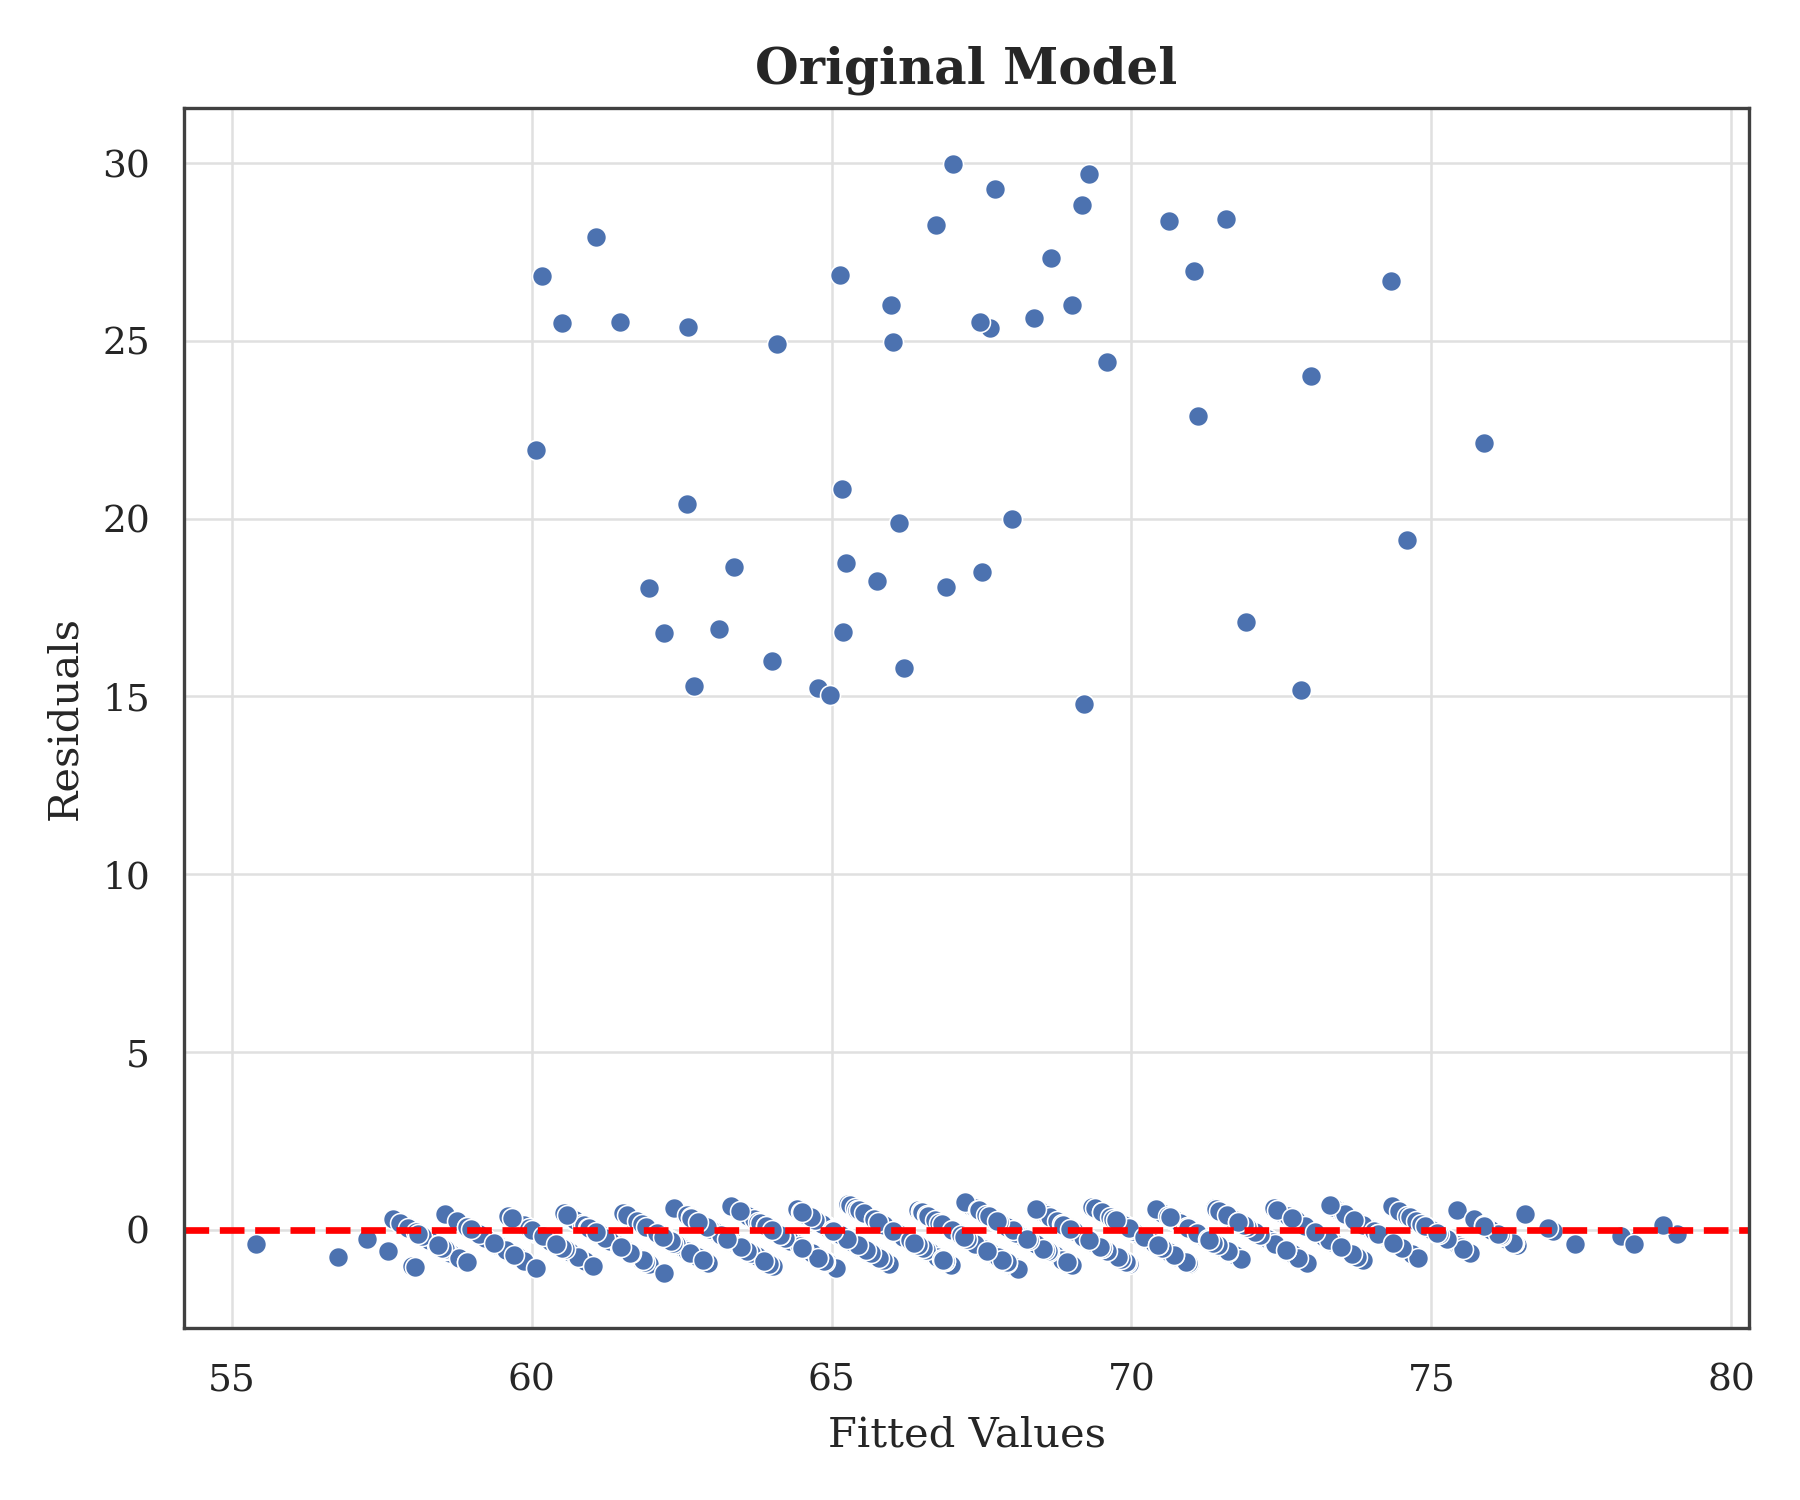
\includegraphics[width=\textwidth]{../figs/ols_residuals_fitted_original.png}
    \caption{Original OLS model}
\end{subfigure}
\hfill
\begin{subfigure}{0.48\textwidth}
    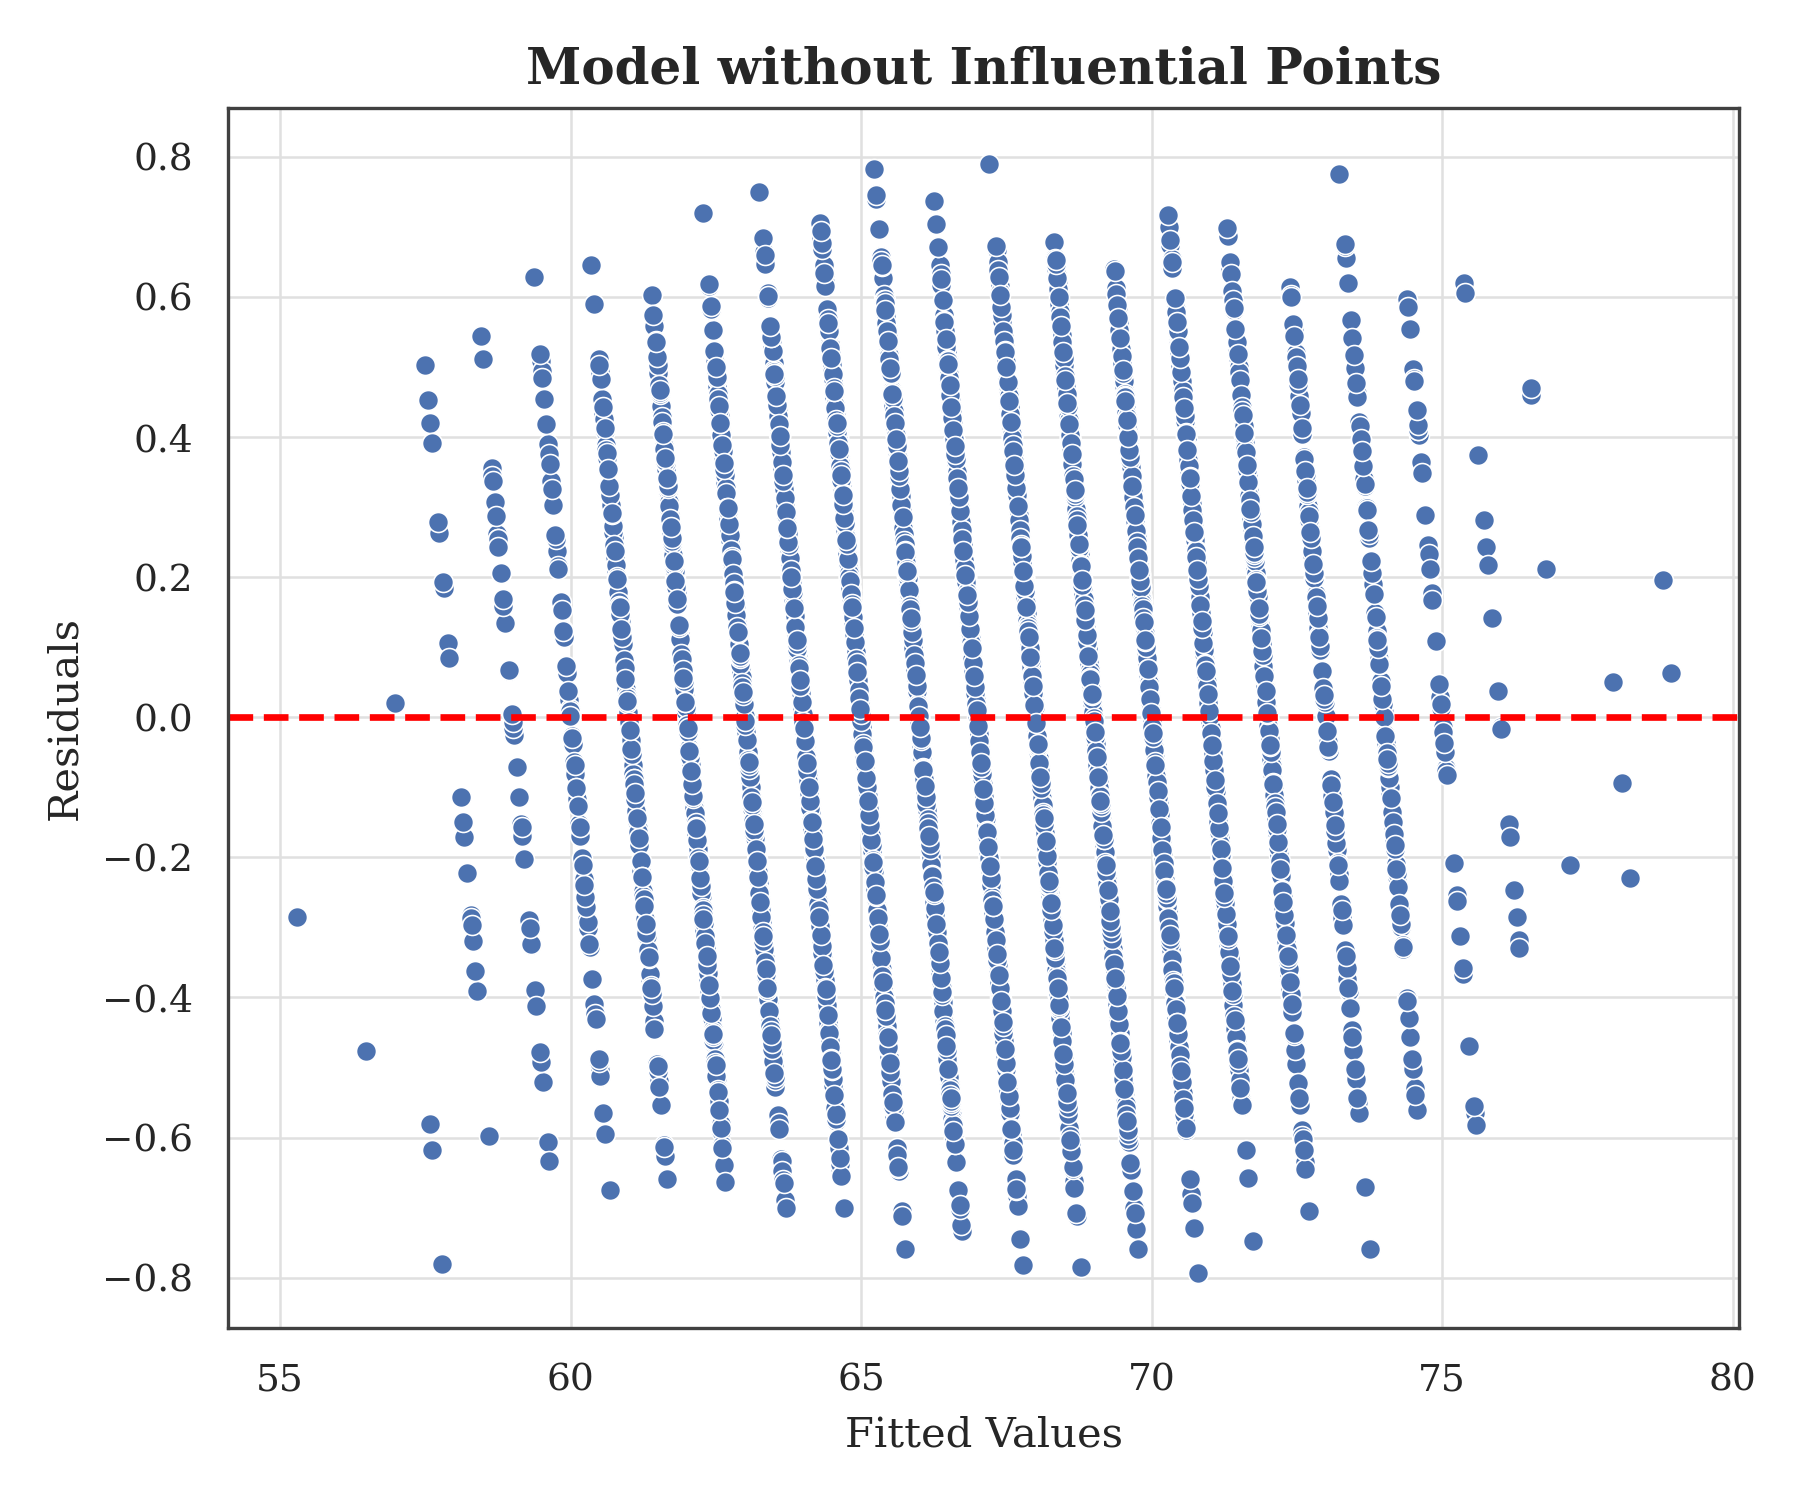
\includegraphics[width=\textwidth]{../figs/ols_residuals_fitted_no_influential.png}
    \caption{After removing influential points}
\end{subfigure}
\caption{Residual diagnostics before and after removing influential observations in OLS.}
\label{fig:ols_residual_compare}
\end{figure}



\section{Discussion}


Under the causal assumptions, the OLS outcome regression suggests a positive effect of extracurricular activity participation on exam performance. After controlling all the covariates, students who participate in extracurricular activities are estimated to score approximately 0.56 points higher on average than students who do not participate.The robustness checks indicate that while the magnitude of the estimated effect is sensitive to influential observations, the overall conclusion of a positive effect remains consistent. 

Several limitations should be acknowledged. First, because the data are observational rather than experimental, the unobserved confounding bias may still exist if there are relevant factors that influence both treatment assignment and outcomes that are not included in the model. Moreover, the regression models rely on linearity and functional form assumptions. Although residual diagnostics and robustness checks were conducted, model misspecification may still exist if the true relationships are nonlinear or involve more complex interactions.


\section{Conclusion}


This project investigated the relationship between extracurricular activity participation and academic performance using observational student-level data. Using OLS outcome regression with covariate adjustment, we find evidence of a positive association between extracurricular participation and exam scores. The estimated treatment effect remains positive after diagnostic checks and robustness analyses, supporting the stability of the main findings.

Additional analyses, including treatment effect heterogeneity and inverse probability weighting, are presented in Section~\ref{sec:additional-work}. These supplementary analyses provide further robustness checks for the main conclusions. In particular, we do not find strong statistical evidence that the treatment effect varies substantially by motivation level or study hours, and the weighted estimates are broadly consistent with the primary OLS results.

Overall, the findings suggest that participation in extracurricular activities may have a modest positive effect on academic performance, although the causal interpretation remains subject to the assumptions and limitations inherent in observational studies.


\newpage
\section{Additional Work}\label{sec:additional-work}

In this section, we explore potential treatment effect heterogeneity by including interaction terms between the treatment and selected covariates. We also implement inverse probability weighting (IPW) based on propensity scores to further adjust for confounding bias and compare the results with the OLS estimates. Both methods are conducted with and without influential observations to assess the robustness of the findings.

\subsection{Treatment Effect Heterogeneity}

\subsubsection{Model Specification}

To explore treatment effect heterogeneity, we extend the model by including interaction terms between treatment and selected covariates. This allows the treatment effect to vary across subgroups while maintaining the same identification assumptions.


\begin{equation*}
Y_i = \alpha_0 + \alpha_1 T_i + X_i^T \alpha + (T_i \cdot X_i)^T \gamma + \epsilon_i
\end{equation*}

where $\gamma$ captures the heterogeneity in treatment effects across different levels of covariates. After exploration, we select two covariates (Hours studied and Motivation level) to include in the interaction terms, as they show the largest imbalance between treatment and control groups qualitatively and are also theoretically relevant to the relationship between extracurricular activities and exam scores.Visualizations of the interaction patterns are provided in Figures~\ref{fig:cat_interactions} and~\ref{fig:num_interactions} in the Appendix~\ref{sec:interation-plot}. 

\subsubsection{Estimation and Interpretation}
Following the same way as the main effect model, we provide the coefficient estimates for the interaction model both with and without influential observations. Details of the coefficient estimates are shown in Table~\ref{tab:interaction-effects}. For the categorical variable motivation level, we use the high motivation group as the reference category. For the continuous variable hours studied, the coefficient represents the change in treatment effect for each additional hour studied.

\begin{table}[htbp]
\centering
\caption{Heterogeneous Treatment Effects with and without Influential Observations}
\label{tab:interaction-effects}
\begin{tabular}{lccc ccc}
\toprule
& \multicolumn{3}{c}{With influentials} & \multicolumn{3}{c}{Without influentials} \\
\cmidrule(lr){2-4} \cmidrule(lr){5-7}
Term & Coef. & 95\% CI & p-value & Coef. & 95\% CI & p-value \\
\midrule
Extracurricular Activities 
& 0.921 & [0.505, 1.337] & $<$0.001 
& 0.489 & [0.425, 0.553] & $<$0.001 \\

$\times$ Motivation (Low) 
& -0.250 & [-0.551, 0.052] & 0.104 
& -0.040 & [-0.086, 0.007] & 0.094 \\

$\times$ Motivation (Medium) 
& -0.190 & [-0.465, 0.085] & 0.175 
& -0.004 & [-0.046, 0.038] & 0.858 \\

$\times$ Hours Studied 
& -0.009 & [-0.027, 0.008] & 0.287 
& 0.002 & [-0.001, 0.004] & 0.270 \\

\bottomrule
\end{tabular}
\end{table}

\begin{itemize}

\item \textbf{Baseline treatment effect.} 
In the interaction model, the coefficient on extracurricular activities represents the treatment effect for the reference group, i.e., students with high motivation (the omitted category) and zero study hours. The estimated effect is 0.921 (95\% CI: [0.505, 1.337], $p < 0.001$). 

However, the interpretation at zero study hours is not substantively meaningful, as the minimum value in the dataset is 1. Therefore, this coefficient should be viewed primarily as a baseline for interpreting interaction effects rather than a standalone causal estimate.

After removing influential observations, the baseline effect decreases to 0.489 (95\% CI: [0.425, 0.553], $p < 0.001$), indicating that the magnitude of the estimated effect is sensitive to influential data points, although the positive effect remains robust.

\item \textbf{Interaction with motivation level.} 
The interaction terms capture how the treatment effect differs across motivation levels relative to the high-motivation group. The estimated interaction coefficients are -0.250 for low motivation and -0.190 for medium motivation. This implies that the treatment effect is smaller for students with lower motivation.

For example, holding study hours fixed at zero (for comparison), the implied treatment effects are:
\begin{itemize}
    \item High motivation: 0.921
    \item Medium motivation: $0.921 - 0.190 = 0.731$
    \item Low motivation: $0.921 - 0.250 = 0.671$
\end{itemize}

While these point estimates suggest that highly motivated students may benefit more from extracurricular activities, both interaction terms are statistically insignificant at the 5\% level. Therefore, there is no strong empirical evidence that the treatment effect varies systematically by motivation level.

After removing influential observations, the interaction effects shrink substantially toward zero and remain statistically insignificant, further indicating that the evidence for heterogeneity by motivation level is weak and not robust.

\item \textbf{Interaction with study hours.} 
The interaction between extracurricular participation and study hours is estimated as -0.009 ($p = 0.287$). This implies that the treatment effect varies with study hours according to:

\[
\text{Heterogeneous Treatment Effect} = 0.921 - 0.009 \times \text{Hours Studied}.
\]

This suggests a negative relationship between study time and the marginal benefit of extracurricular activities, potentially reflecting a substitution effect between academic effort and extracurricular engagement.

However, the interaction term is not statistically significant, indicating that there is no strong evidence that the treatment effect varies with study hours. After removing influential observations, the interaction coefficient becomes even closer to zero and remains insignificant, reinforcing the conclusion that the heterogeneous effect is not supported by the data.
\end{itemize}





% \paragraph{Model Diagnostics}

% We carry out the same diagnostic checks for the interaction model as we did for the main effect model. After moving the influential observations, the residual patterns show improved symmetry and reduced heteroskedasticity. We see high VIF in the interaction terms with treament variable. But for other covaraites, the VIF values are still below 5, indicating no severe multicollinearity. 

\subsection{Propensity Score and WLS}

\subsubsection{Model Specification}

Propensity score measures the probability of receiving treatment given the observed covariates. By estimating the propensity score, we can create a weighted dataset that mimics a randomized experiment, where the distribution of covariates is balanced between the treatment and control groups. In practice, we use logistic regression to estimate the propensity score and then apply the weights to estimate the ATE using weighted least squares (WLS) regression.

The propensity score model is specified as:
\begin{equation*}
P(T_i = 1 \mid X_i) = \frac{\exp(\beta_0 + X_i^T \beta)}{1 + \exp(\beta_0 + X_i^T \beta)}
\end{equation*}

The WLS model is then specified as:
\begin{equation*}
Y_i = \alpha_0 + \alpha_1 T_i + X_i^\top \alpha + \epsilon_i
\end{equation*}
where the weights are defined as:
\begin{equation*}w_i = \frac{T_i}{P(T_i = 1 \mid X_i)} + \frac{1 - T_i}{1 - P(T_i = 1 \mid X_i)}\end{equation*}

\subsubsection{Propensity Score Evaluation}
\begin{itemize}
    \item \textbf{Model Fit}: With all the covariates included, the logistic regression model for the propensity score shows poor fit, with a pseudo-$R^2$ of 0.003 and all the covariates being statistically insignificant at the 5\% level. This suggests that the observed covariates do not strongly predict treatment assignment, which may indicate that the unconfoundedness assumption is more plausible in this context.
    \item \textbf{Covariate Balance}: After applying the inverse probability weights, we reassess the balance of covariates between the treatment and control groups. Figure \ref{fig:balance_ipw} shows all the standardized mean differences becomes much smaller after weighting compared with the unweighted sample. Althought for unweighted sample, the largest SMD is already below the common threshold of 0.1, the weighted sample shows even better balance with all SMDs close to zero, indicating that the IPW approach has successfully balanced the covariates between the treatment and control groups.
    
    \item \textbf{Overlap Assessment}: We examine the distribution of propensity scores to ensure sufficient overlap between the treatment and control groups. The distribution in Figure \ref{fig:ps_distribution} shows the propensities are well distributed across the treatment and control groups.
\end{itemize}


\begin{figure}[htbp]
    \centering
    \caption{Propensity Score Diagnostics}

    \begin{subfigure}{0.45\textwidth}
            \centering
        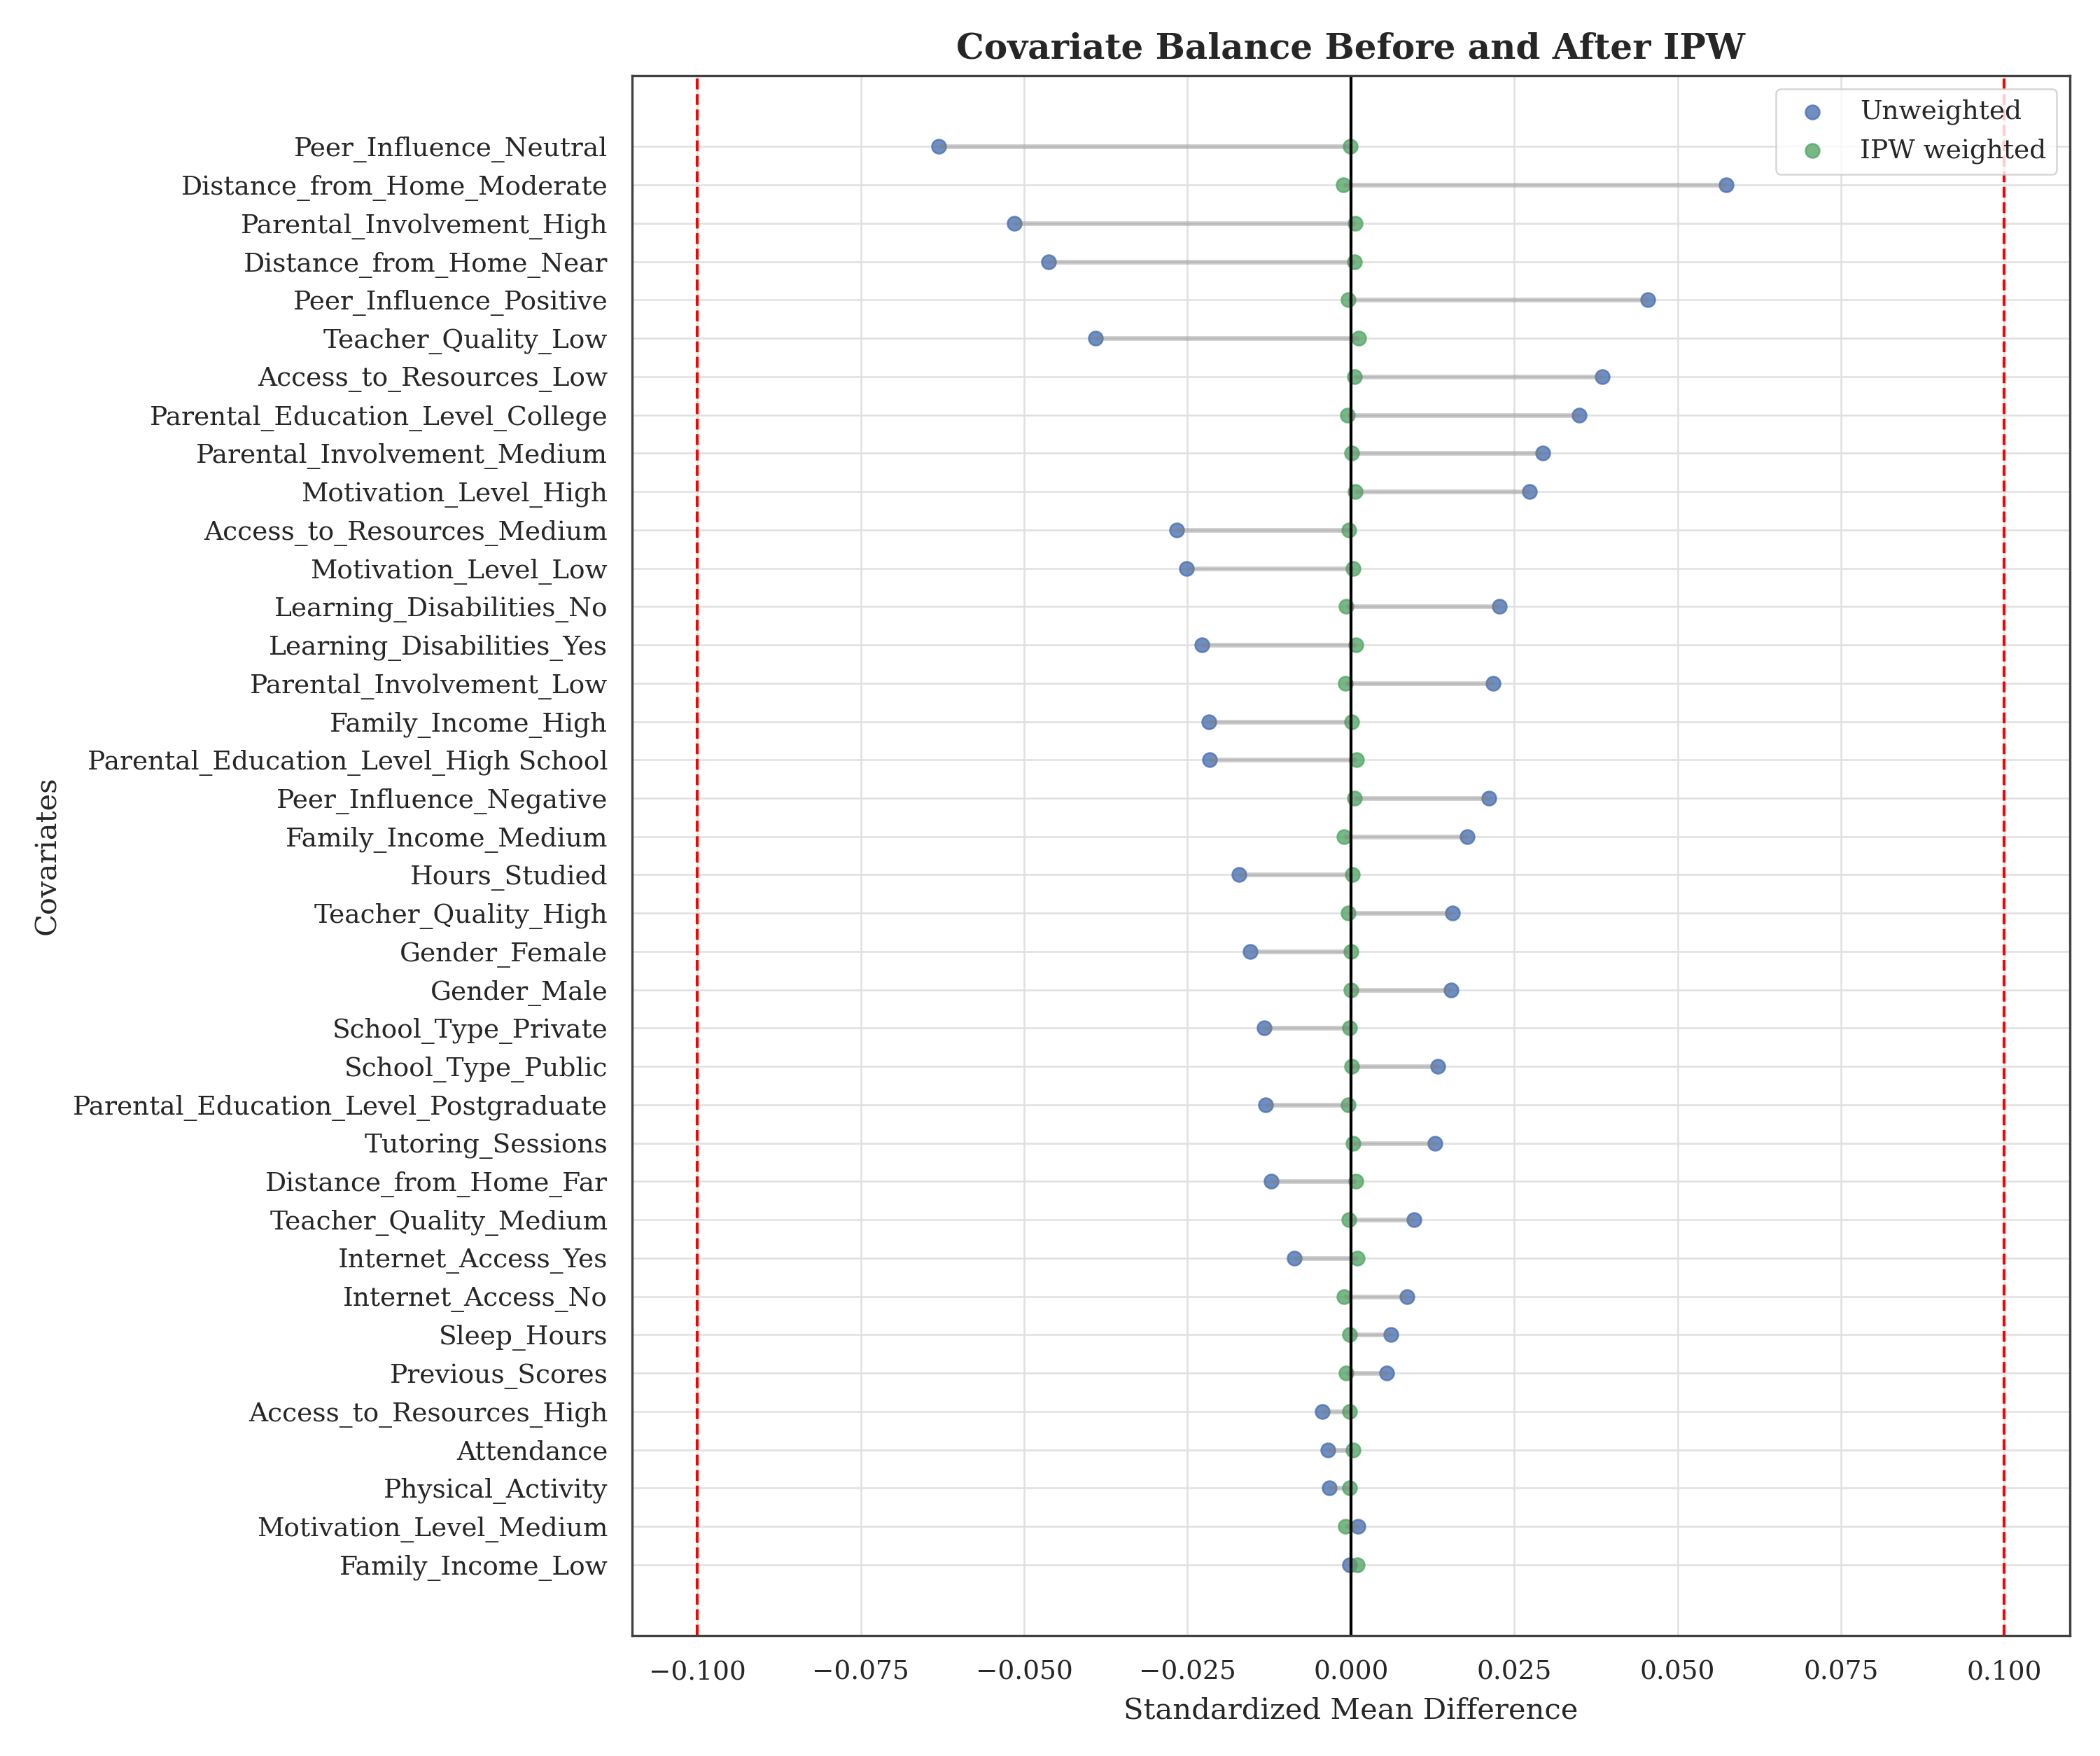
\includegraphics[width=\textwidth]{../figs/balance_ipw.png}
        \caption{Covariate Balance Before and After IPW}
        \label{fig:balance_ipw}
    \end{subfigure}
    \hfill
    \begin{subfigure}{0.45\textwidth}
        \centering
        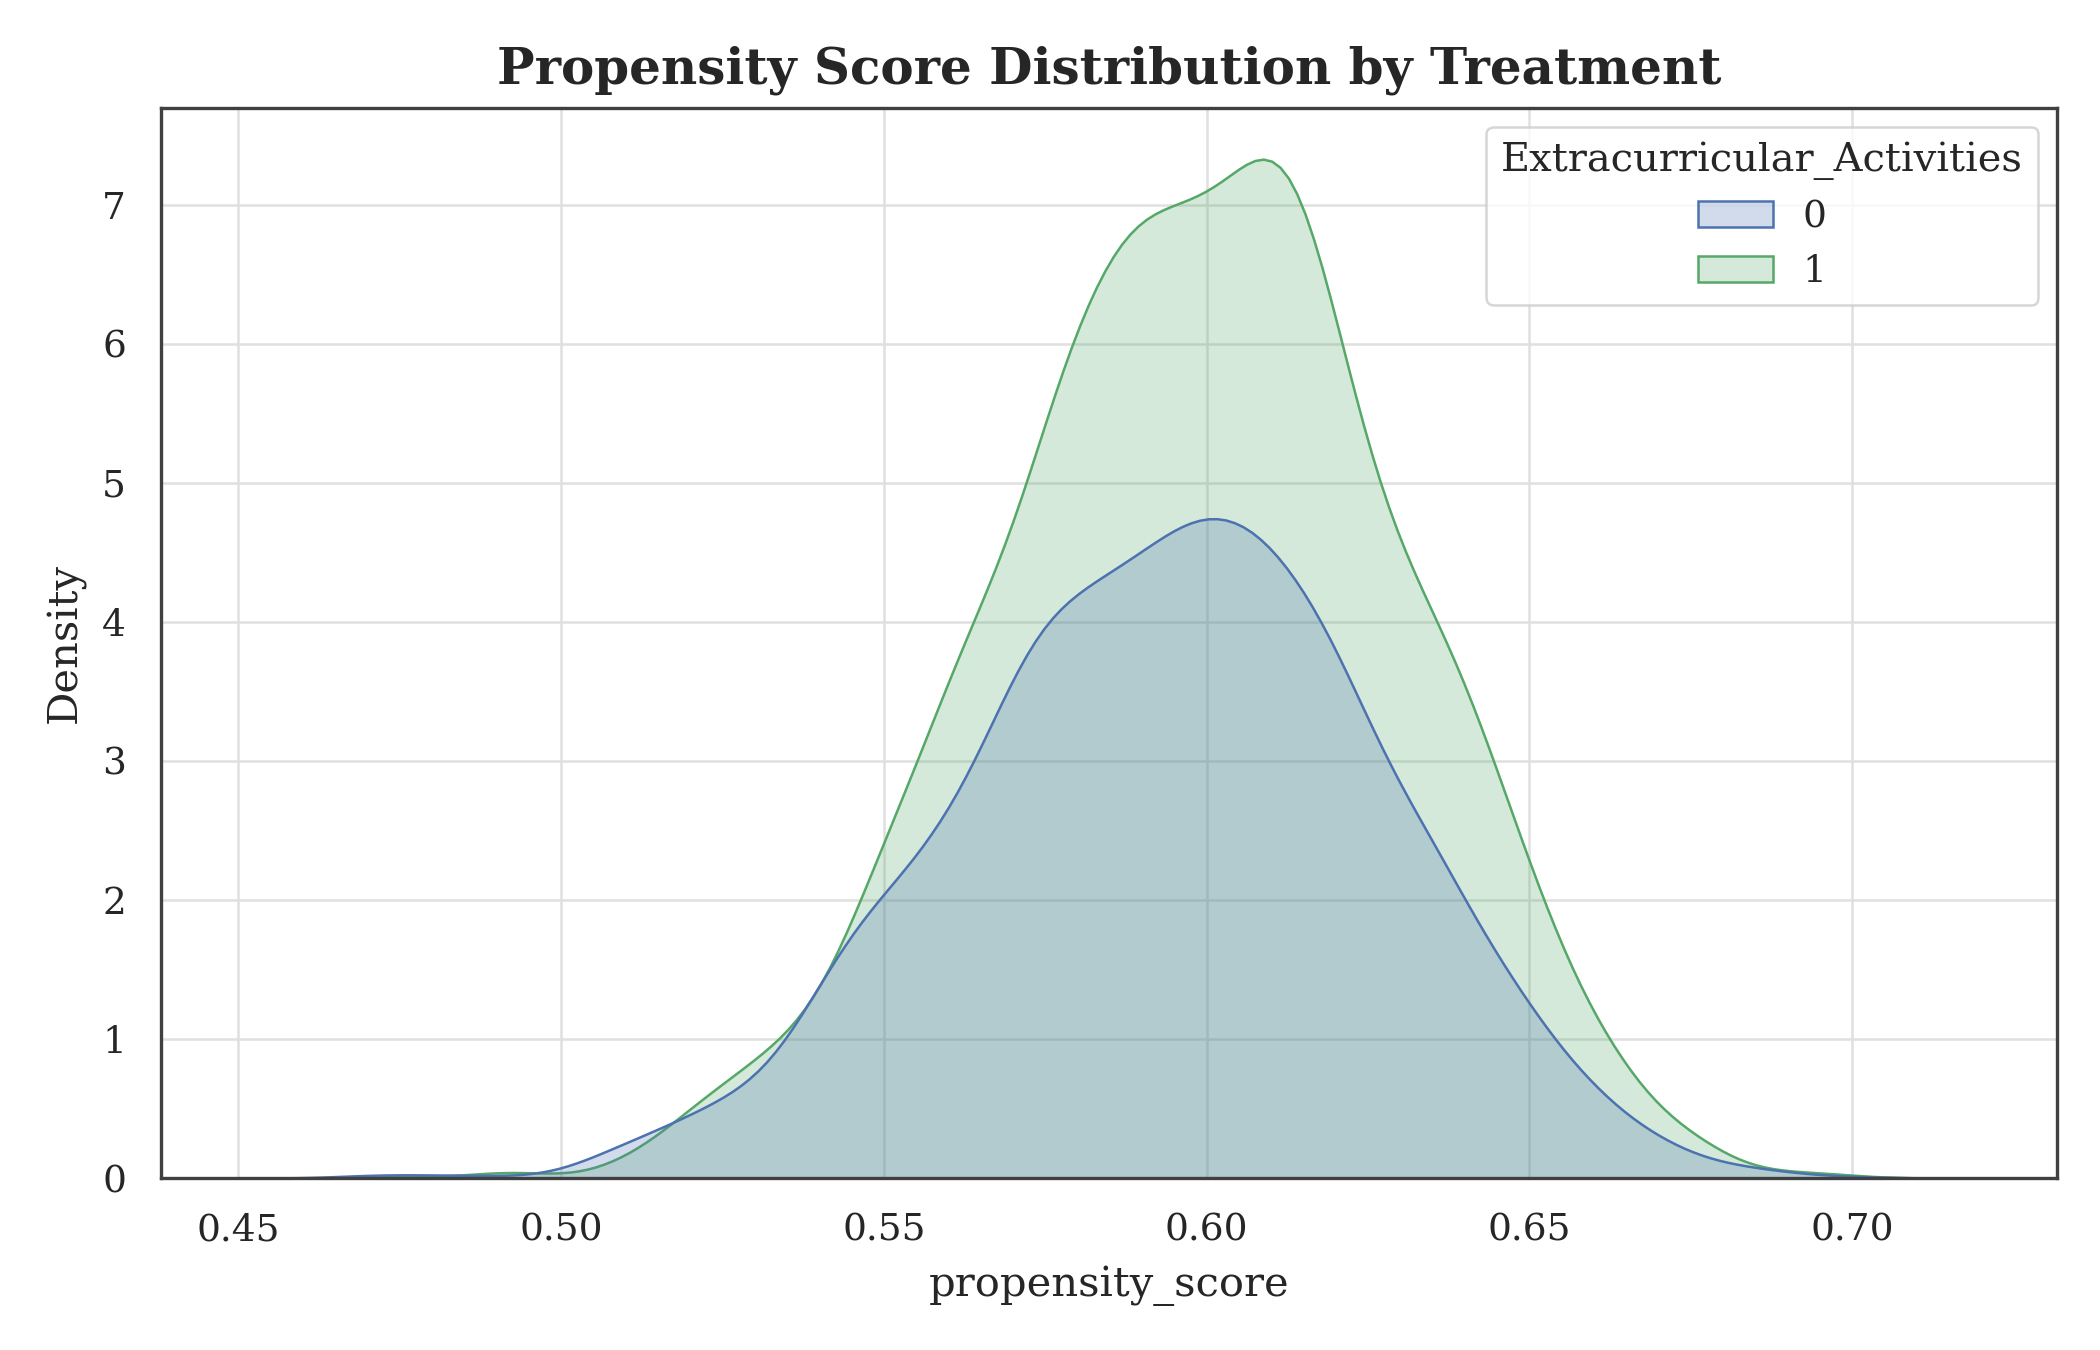
\includegraphics[width=\textwidth]{../figs/ps_distribution.png}
        \caption{Distribution of Propensity Scores by Treatment Group}
        \label{fig:ps_distribution}
    \end{subfigure}

\end{figure}

The poor fit of the propensity score model gives us some confidence that the unconfoundedness assumption may hold, as the treatment assignment does not appear to be strongly driven by the observed covariates. The improved balance after weighting also supports the validity of the IPW approach for estimating the causal effect.

\subsubsection{Estimation}

We apply the inverse probability weights to estimate the ATE using weighted least squares regression. The results are shown in Table~\ref{tab:ipw-results}. The estimated treatment effect is 0.562 (95\% CI: [0.462, 0.662], $p < 0.001$) when including all observations, which is consistent with the OLS estimate. After removing influential observations, the estimated effect decreases to 0.505 (95\% CI: [0.490, 0.521], $p < 0.001$), indicating that influential points have a noticeable impact on the magnitude of the estimated effect, although the positive association remains robust. 

The 95\% confidence intervals in baseline outcome regression and IPW are quite similar, even the same after removing influential observations, which suggests that the IPW approach is providing a similar estimate of the treatment effect as the OLS model, lending credibility to the causal interpretation under the unconfoundedness assumption.

\begin{table}[htbp]
\centering
\caption{Inverse Probability Weighted (IPW) Estimates with and without Influential Observations}
\label{tab:ipw-results}
\begin{tabular}{lccccc}
\toprule
Model & Effect & Std. Err. & 95\% CI & p-value & $N$ \\
\midrule
With influential observations 
& 0.562 & 0.051 & [0.462, 0.662] & $<$0.001 & 6378 \\

Without influential observations 
& 0.505 & 0.008 & [0.490, 0.521] & $<$0.001 & 6323 \\

\bottomrule
\end{tabular}
\end{table}


% \subsubsection{Model Diagnostics}

% To assess the validity of the OLS assumptions, we examine residual patterns and potential influence of individual observations.

% \paragraph{Residual Analysis}

% The residual-versus-fitted plot in Figure~\ref{fig:ols_residual_compare} (left panel) reveals a distinct group of observations with large positive residuals, suggesting that the model may not fit well for a subset of the data. This pattern may arise from either outliers or model misspecification.

% \paragraph{Influence Diagnostics}

% To further investigate, we compute influence measures based on leverage, and Cook’s distance. Using common thresholds ($4/N$ for Cook’s distance and $\frac{2p}{N}$ for leverage ), approximately 0.9\% of observations are identified as potentially influential. As shown in Figure~\ref{fig:ols-influence}, only a small number of observations exhibit relatively large Cook’s distance values, with the maximum around 0.05, indicating moderate influence.

% \paragraph{Robustness to Influential Observations}

% To evaluate the impact of those influential observations, we refit the model after excluding the identified influential points. The resulting residual plot (Figure~\ref{fig:ols_residual_compare}, right panel) shows a more symmetric and random distribution around zero, suggesting improved model fit and more plausible homoskedasticity.


% \begin{figure}[htbp]
% \centering
% \begin{subfigure}{0.48\textwidth}
%     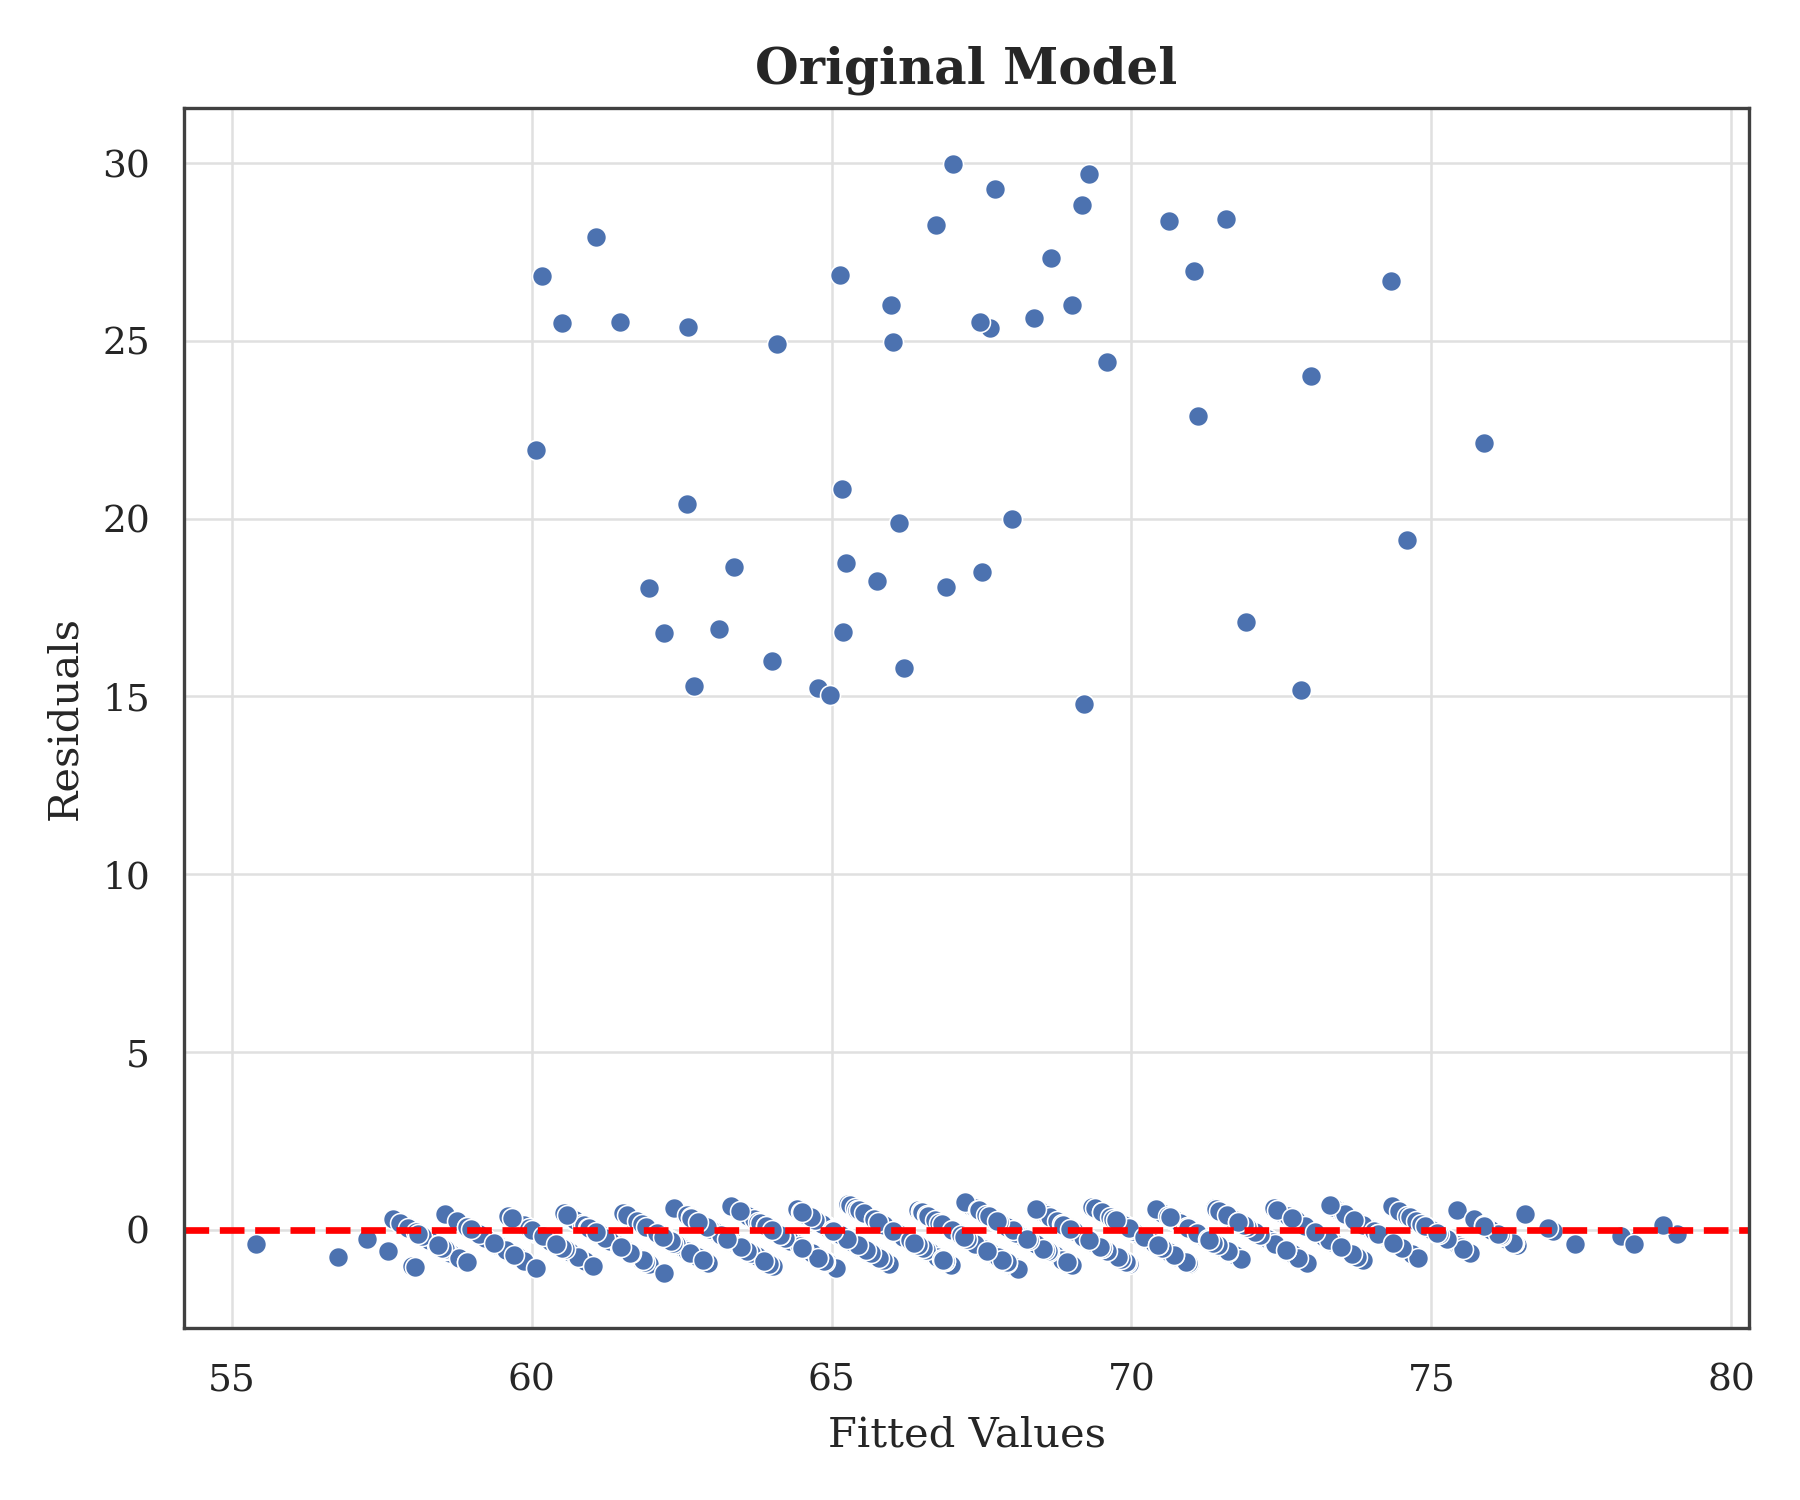
\includegraphics[width=\textwidth]{../figs/ols_residuals_fitted_original.png}
%     \caption{Original OLS model}
% \end{subfigure}
% \hfill
% \begin{subfigure}{0.48\textwidth}
%     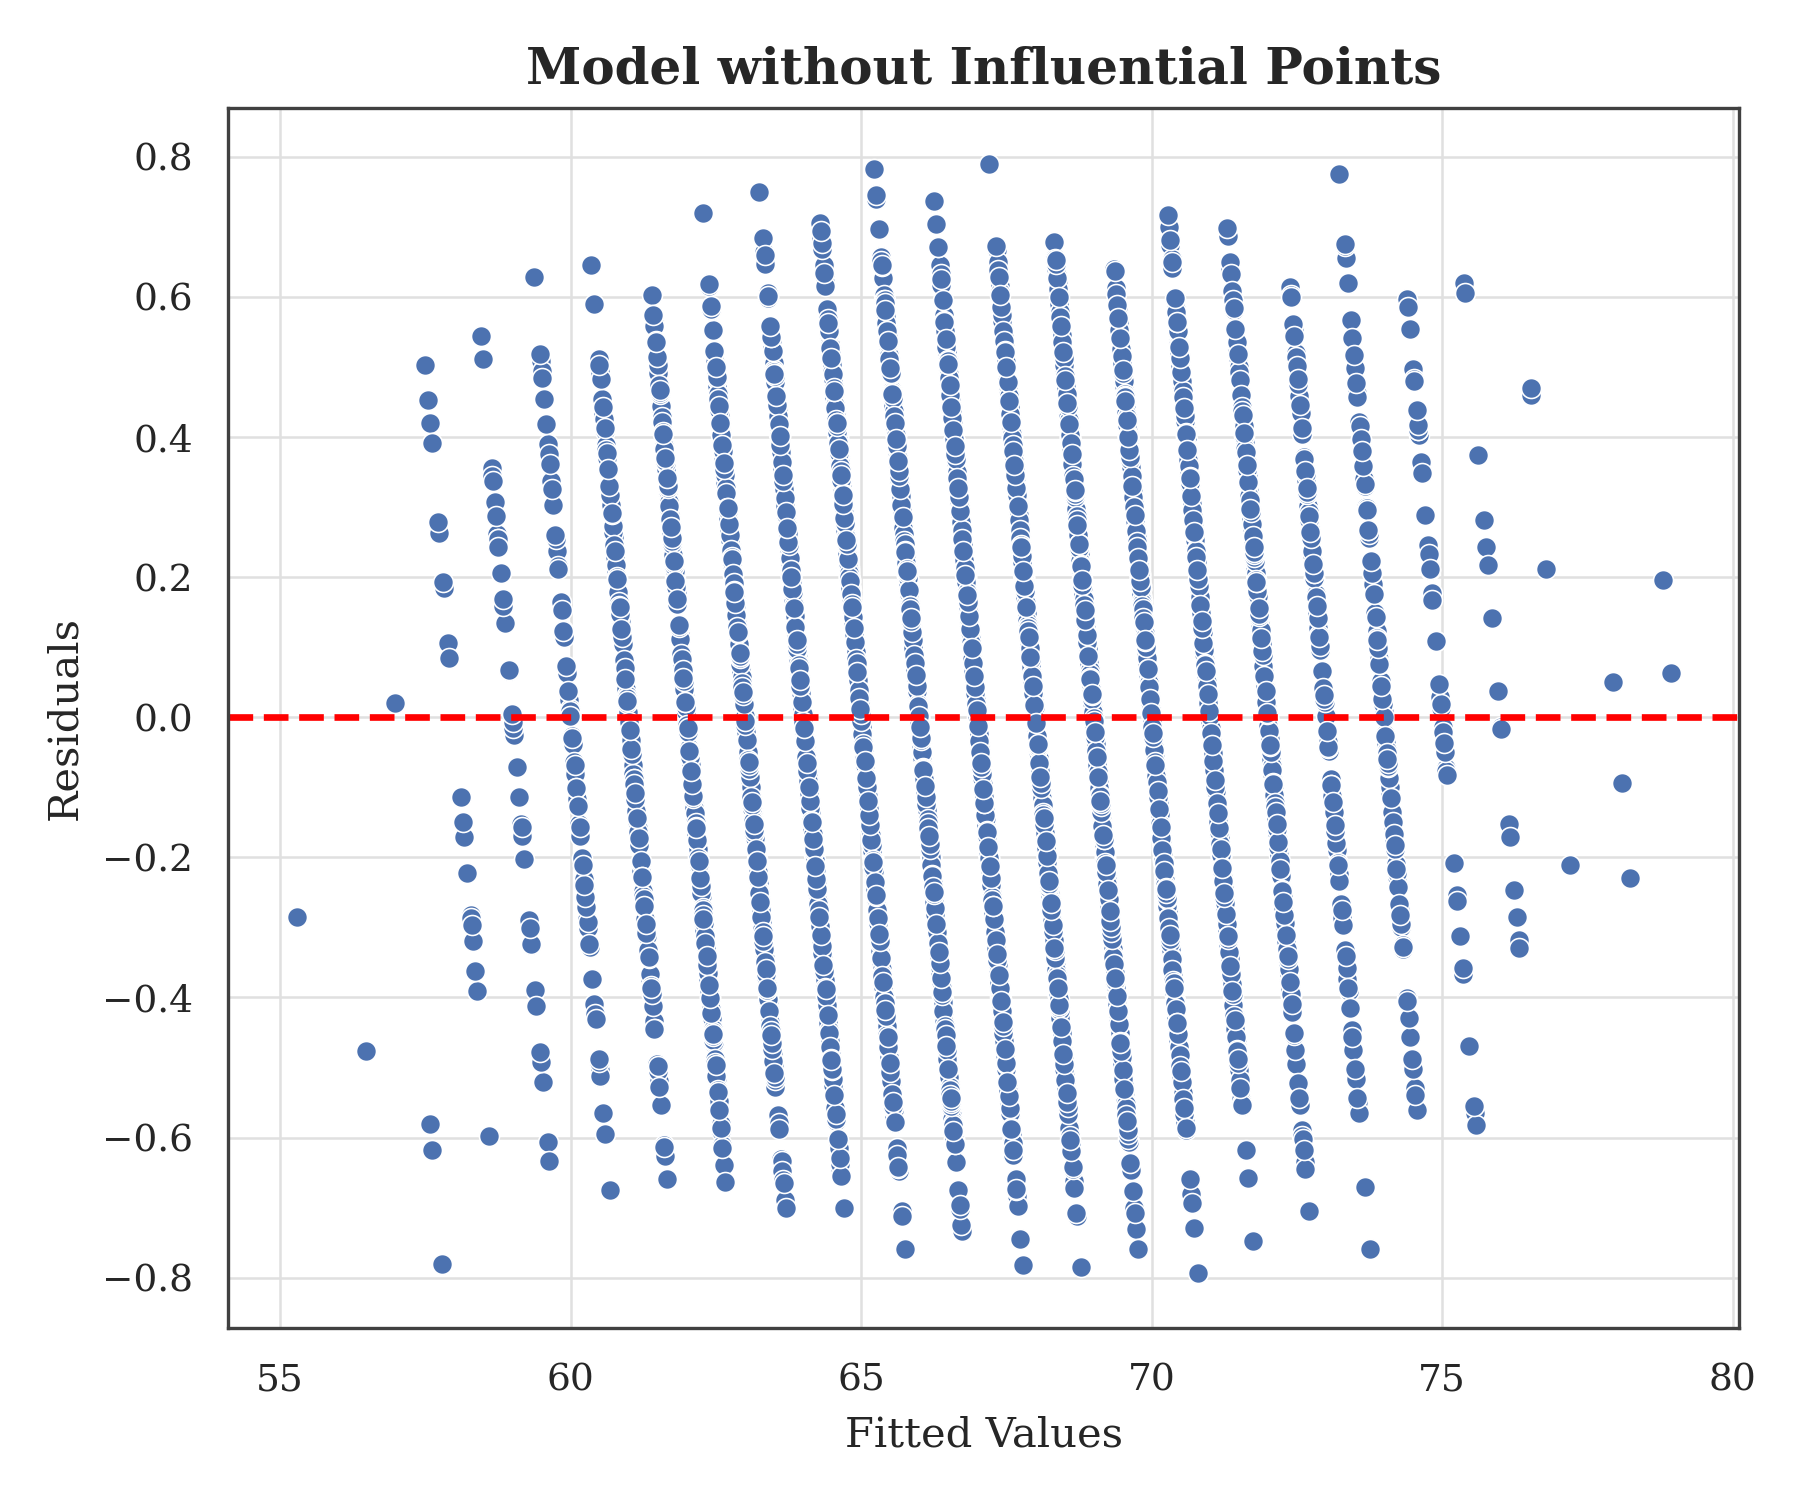
\includegraphics[width=\textwidth]{../figs/ols_residuals_fitted_no_influential.png}
%     \caption{After removing influential points}
% \end{subfigure}
% \caption{Residual diagnostics before and after removing influential observations in OLS.}
% \label{fig:ols_residual_compare}
% \end{figure}

% \begin{figure}[H]
% \centering
% 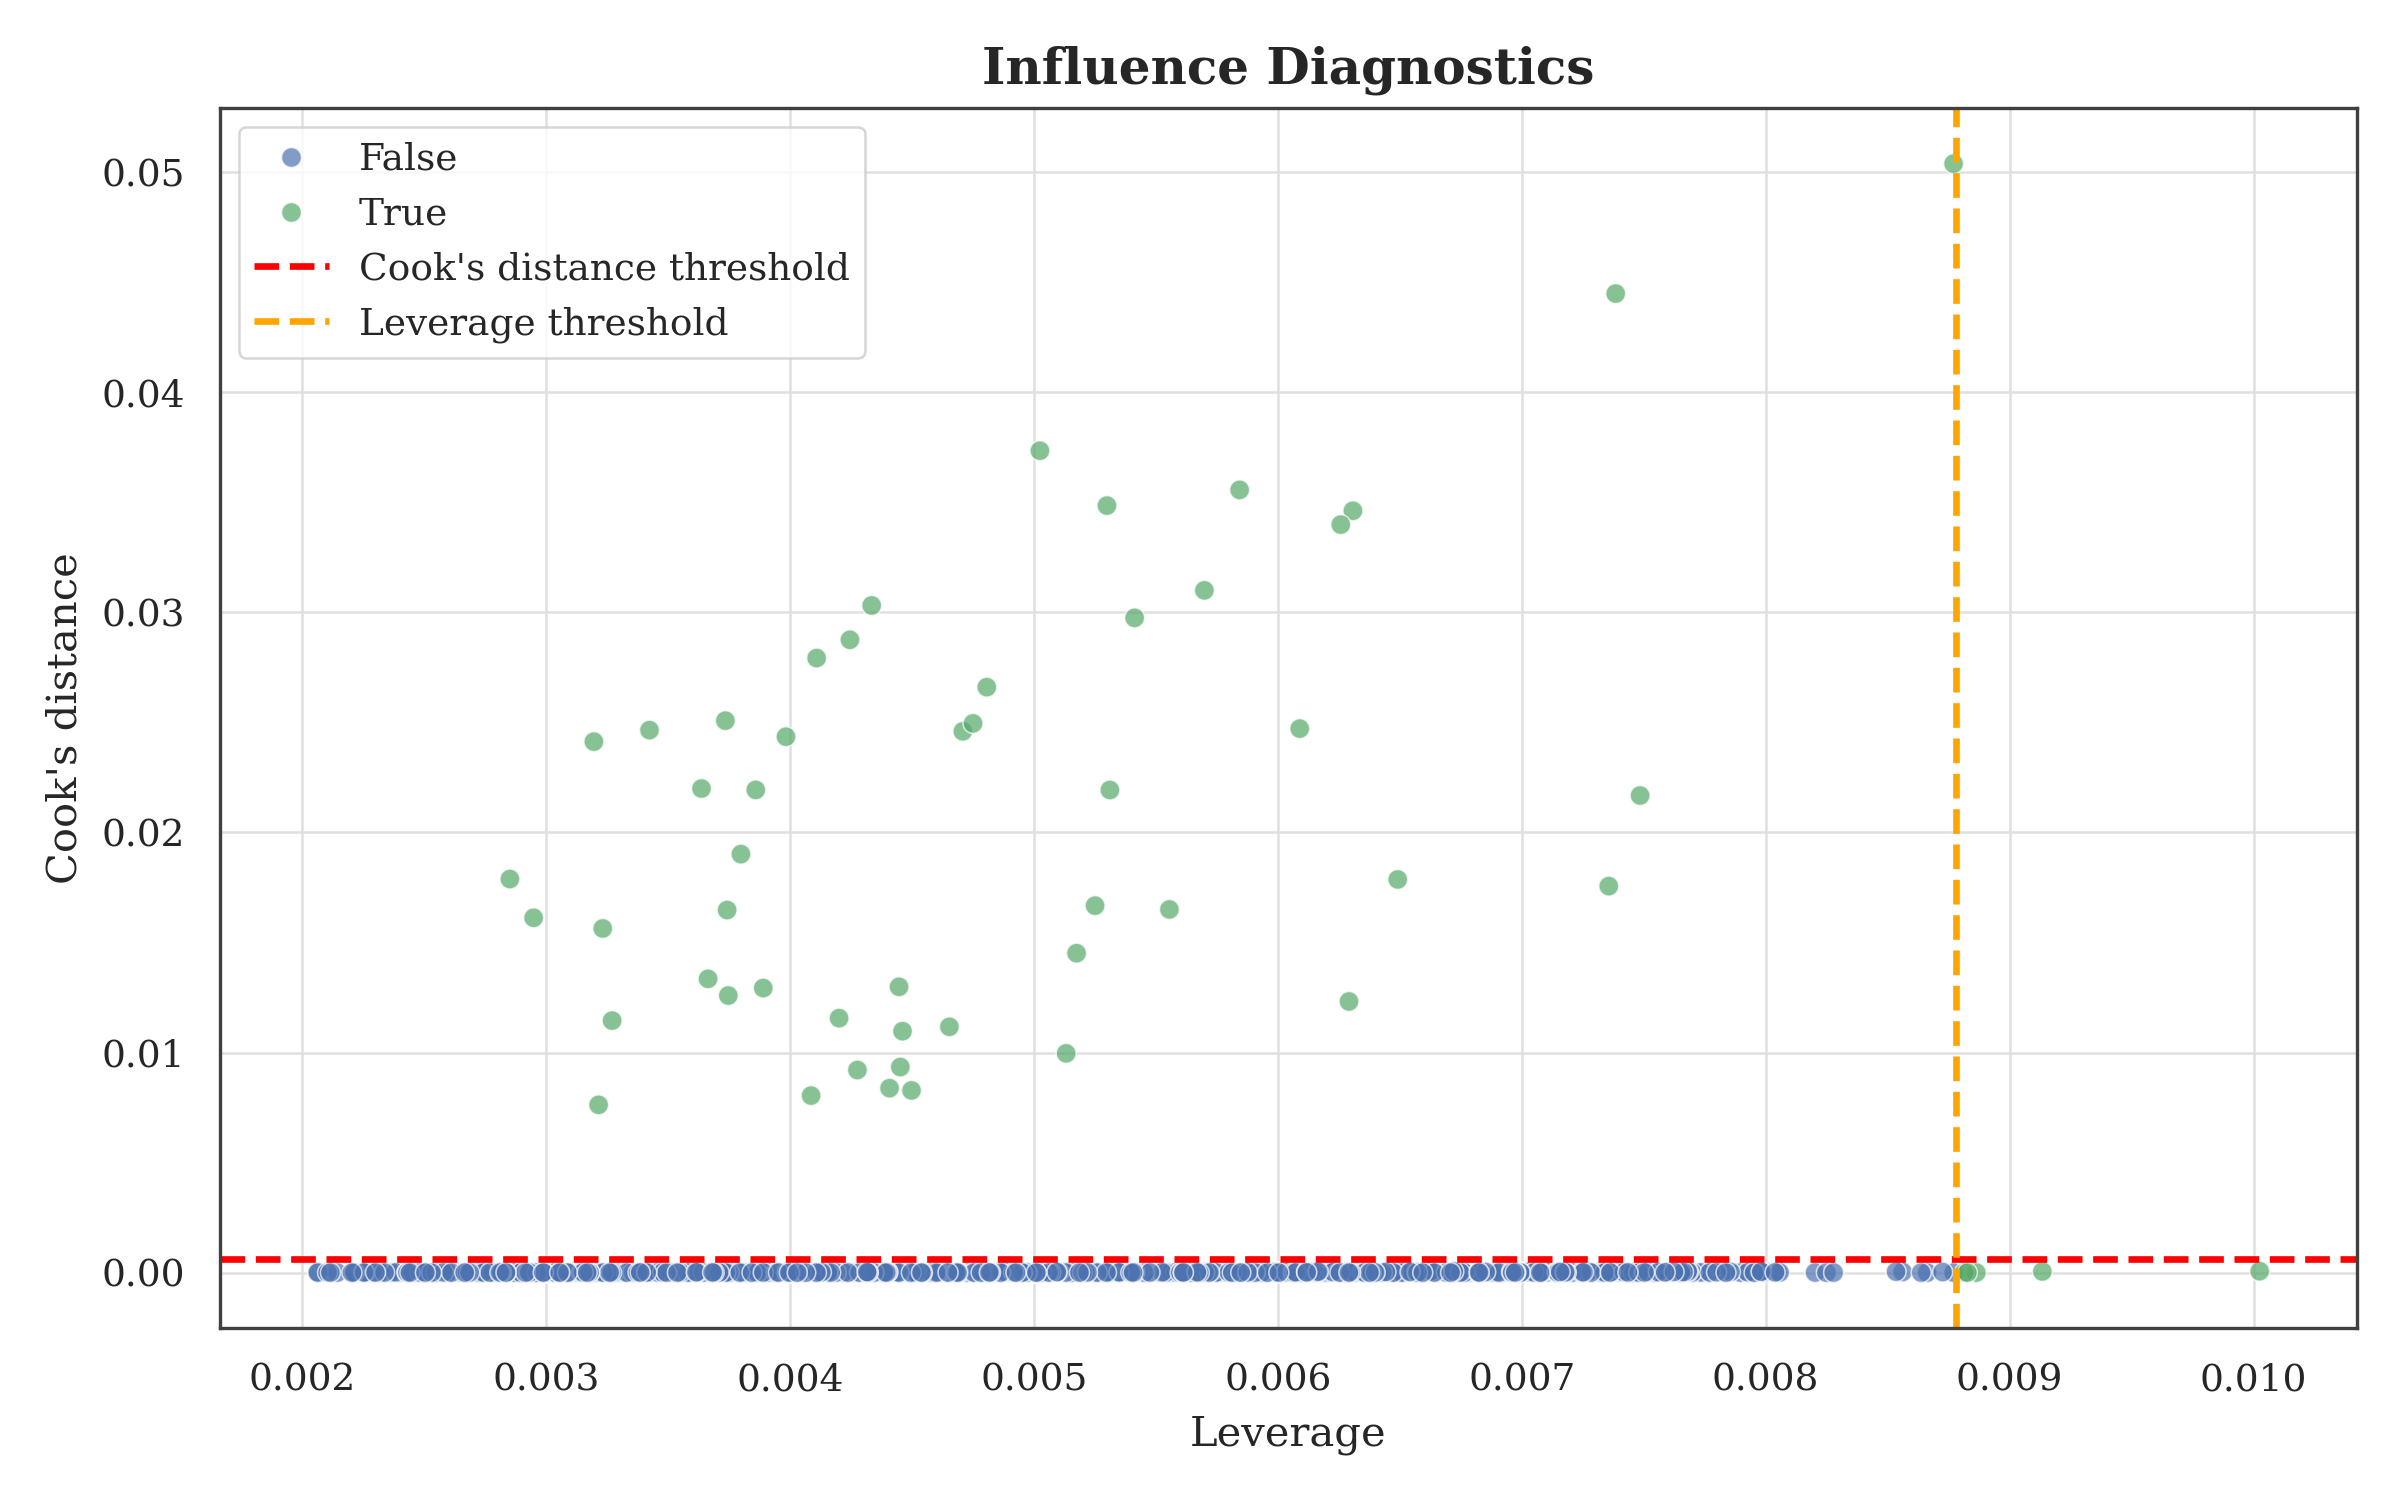
\includegraphics[width=0.75\textwidth]{../figs/ols_influence_diagnostics.png}
% \caption{Influence diagnostics for OLS model based on leverage and Cook's distance. The dashed lines indicate common thresholds for identifying influential observations.}
% \label{fig:ols-influence}
% \end{figure}

% Table~\ref{tab:ols-no-influential} reports the updated coefficient estimates. The estimated main effect remains positive and statistically significant, with a slightly reduced magnitude (0.506 compared to 0.562) and a narrower confidence interval. This indicates that while influential observations affect the magnitude of the estimate, the overall conclusion is robust. For the downstream exploration, we keep the whole data for analysis since first we have little prior information about the influential observations and the ratio is quite small and acceptable. However, we will also report the results after removing influential observations for comparison and robustness check.

% \begin{table}[htbp]
% \centering
% \caption{OLS Estimate After Removing Influential Observations}
% \label{tab:ols-no-influential}
% \begin{tabular}{lccccccc}
% \toprule
% Effect & Std. Err. & p-value & CI Lower & CI Upper & $R^2$ & Adj. $R^2$ & $N$ \\
% \midrule
% 0.506 & 0.008 & $<$0.001 & 0.490 & 0.521 & 0.991 & 0.991 & 6323 \\
% \bottomrule
% \end{tabular}
% \end{table}

% \paragraph{Multicollinearity}

% We assess multicollinearity using variance inflation factors (VIF). All VIF values are below 5, with a maximum of 2.826, indicating no evidence of severe multicollinearity. This suggests that the coefficient estimates are stable and not overly sensitive to small perturbations in the data.




% \subsection{Treatment Effect Heterogeneity}

% \subsubsection{Model Specification}

% To explore treatment effect heterogeneity, we extend the model by including interaction terms between treatment and selected covariates. This allows the treatment effect to vary across subgroups while maintaining the same identification assumptions.


% \begin{equation*}
% Y_i = \alpha_0 + \alpha_1 T_i + X_i^T \alpha + (T_i \cdot X_i)^T \gamma + \epsilon_i
% \end{equation*}

% where $\gamma$ captures the heterogeneity in treatment effects across different levels of covariates. After exploration, we select two covariates (\textbf{Hours studied} and \textbf{Motivation level}) to include in the interaction terms, as they show the largest imbalance between treatment and control groups qualitatively and are also theoretically relevant to the relationship between extracurricular activities and exam scores.Visualizations of the interaction patterns are provided in Figures~\ref{fig:cat_interactions} and~\ref{fig:num_interactions} in the Appendix.

% \subsubsection{Result}

% Following the same way as the main effect model, we provide the coefficient estimates for the interaction model both with and without influential observations, followed by the model diagnostics for residual patterns and multicollinearity.

% \subsubsection{Interpretation}

% Details of the coefficient estimates are shown in Table~\ref{tab:interaction-effects}. For the categorical variable motivation level, we use the high motivation group as the reference category. For the continuous variable hours studied, the coefficient represents the change in treatment effect for each additional hour studied.


% \begin{itemize}

% \item \textbf{Baseline treatment effect.} 
% In the interaction model, the coefficient on extracurricular activities represents the treatment effect for the reference group, i.e., students with high motivation (the omitted category) and zero study hours. The estimated effect is 0.921 (95\% CI: [0.505, 1.337], $p < 0.001$). 

% However, the interpretation at zero study hours is not substantively meaningful, as the minimum value in the dataset is 1. Therefore, this coefficient should be viewed primarily as a baseline for interpreting interaction effects rather than a standalone causal estimate.

% After removing influential observations, the baseline effect decreases to 0.489 (95\% CI: [0.425, 0.553], $p < 0.001$), indicating that the magnitude of the estimated effect is sensitive to influential data points, although the positive effect remains robust.

% \item \textbf{Interaction with motivation level.} 
% The interaction terms capture how the treatment effect differs across motivation levels relative to the high-motivation group. The estimated interaction coefficients are -0.250 for low motivation and -0.190 for medium motivation. This implies that the treatment effect is smaller for students with lower motivation.

% For example, holding study hours fixed at zero (for comparison), the implied treatment effects are:
% \begin{itemize}
%     \item High motivation: 0.921
%     \item Medium motivation: $0.921 - 0.190 = 0.731$
%     \item Low motivation: $0.921 - 0.250 = 0.671$
% \end{itemize}

% While these point estimates suggest that highly motivated students may benefit more from extracurricular activities, both interaction terms are statistically insignificant at the 5\% level. Therefore, there is no strong empirical evidence that the treatment effect varies systematically by motivation level.

% After removing influential observations, the interaction effects shrink substantially toward zero and remain statistically insignificant, further indicating that the evidence for heterogeneity by motivation level is weak and not robust.

% \item \textbf{Interaction with study hours.} 
% The interaction between extracurricular participation and study hours is estimated as -0.009 ($p = 0.287$). This implies that the treatment effect varies with study hours according to:

% \[
% \text{Heterogeneous Treatment Effect} = 0.921 - 0.009 \times \text{Hours Studied}.
% \]

% This suggests a negative relationship between study time and the marginal benefit of extracurricular activities, potentially reflecting a substitution effect between academic effort and extracurricular engagement.

% However, the interaction term is not statistically significant, indicating that there is no strong evidence that the treatment effect varies with study hours. After removing influential observations, the interaction coefficient becomes even closer to zero and remains insignificant, reinforcing the conclusion that the heterogeneous effect is not supported by the data.
% \end{itemize}





% \begin{table}[htbp]
% \centering
% \caption{Heterogeneous Treatment Effects with and without Influential Observations}
% \label{tab:interaction-effects}
% \begin{tabular}{lccc ccc}
% \toprule
% & \multicolumn{3}{c}{With influentials} & \multicolumn{3}{c}{Without influentials} \\
% \cmidrule(lr){2-4} \cmidrule(lr){5-7}
% Term & Coef. & 95\% CI & p-value & Coef. & 95\% CI & p-value \\
% \midrule
% Extracurricular Activities 
% & 0.921 & [0.505, 1.337] & $<$0.001 
% & 0.489 & [0.425, 0.553] & $<$0.001 \\

% $\times$ Motivation (Low) 
% & -0.250 & [-0.551, 0.052] & 0.104 
% & -0.040 & [-0.086, 0.007] & 0.094 \\

% $\times$ Motivation (Medium) 
% & -0.190 & [-0.465, 0.085] & 0.175 
% & -0.004 & [-0.046, 0.038] & 0.858 \\

% $\times$ Hours Studied 
% & -0.009 & [-0.027, 0.008] & 0.287 
% & 0.002 & [-0.001, 0.004] & 0.270 \\

% \bottomrule
% \end{tabular}
% \end{table}


% \paragraph{Model Diagnostics}

% We carry out the same diagnostic checks for the interaction model as we did for the main effect model. After moving the influential observations, the residual patterns show improved symmetry and reduced heteroskedasticity. We see high VIF in the interaction terms with treament variable. But for other covaraites, the VIF values are still below 5, indicating no severe multicollinearity. 

% \subsection{Propensity Score and WLS}

% \subsubsection{Model Specification}

% Propensity score measures the probability of receiving treatment given the observed covariates. By estimating the propensity score, we can create a weighted dataset that mimics a randomized experiment, where the distribution of covariates is balanced between the treatment and control groups. In practice, we use logistic regression to estimate the propensity score and then apply the weights to estimate the ATE using weighted least squares (WLS) regression.

% The propensity score model is specified as:
% \begin{equation*}
% P(T_i = 1 \mid X_i) = \frac{\exp(\beta_0 + X_i^T \beta)}{1 + \exp(\beta_0 + X_i^T \beta)}
% \end{equation*}

% The WLS model is then specified as:
% \begin{equation*}
% Y_i = \alpha_0 + \alpha_1 T_i + X_i^\top \alpha + \epsilon_i
% \end{equation*}
% where the weights are defined as:
% \begin{equation*}w_i = \frac{T_i}{P(T_i = 1 \mid X_i)} + \frac{1 - T_i}{1 - P(T_i = 1 \mid X_i)}\end{equation*}

% \subsubsection{Result}

% \subsubsection{Propensity Score Evaluation}
% \begin{itemize}
%     \item \textbf{Model Fit}: With all the covariates included, the logistic regression model for the propensity score shows poor fit, with a pseudo-$R^2$ of 0.003 and all the covariates being statistically insignificant at the 5\% level. This suggests that the observed covariates do not strongly predict treatment assignment, which may indicate that the unconfoundedness assumption is more plausible in this context.
%     \item \textbf{Covariate Balance}: After applying the inverse probability weights, we reassess the balance of covariates between the treatment and control groups. Figure \ref{fig:balance_ipw} shows all the standardized mean differences becomes much smaller after weighting compared with the unweighted sample. Althought for unweighted sample, the largest SMD is already below the common threshold of 0.1, the weighted sample shows even better balance with all SMDs close to zero, indicating that the IPW approach has successfully balanced the covariates between the treatment and control groups.
    
%     \item \textbf{Overlap Assessment}: We examine the distribution of propensity scores to ensure sufficient overlap between the treatment and control groups. The distribution in Figure \ref{fig:ps_distribution} shows the propensities are well distributed across the treatment and control groups.
% \end{itemize}


% \begin{figure}[htbp]
%     \centering
%     \caption{Propensity Score Diagnostics}

%     \begin{subfigure}{0.45\textwidth}
%             \centering
%         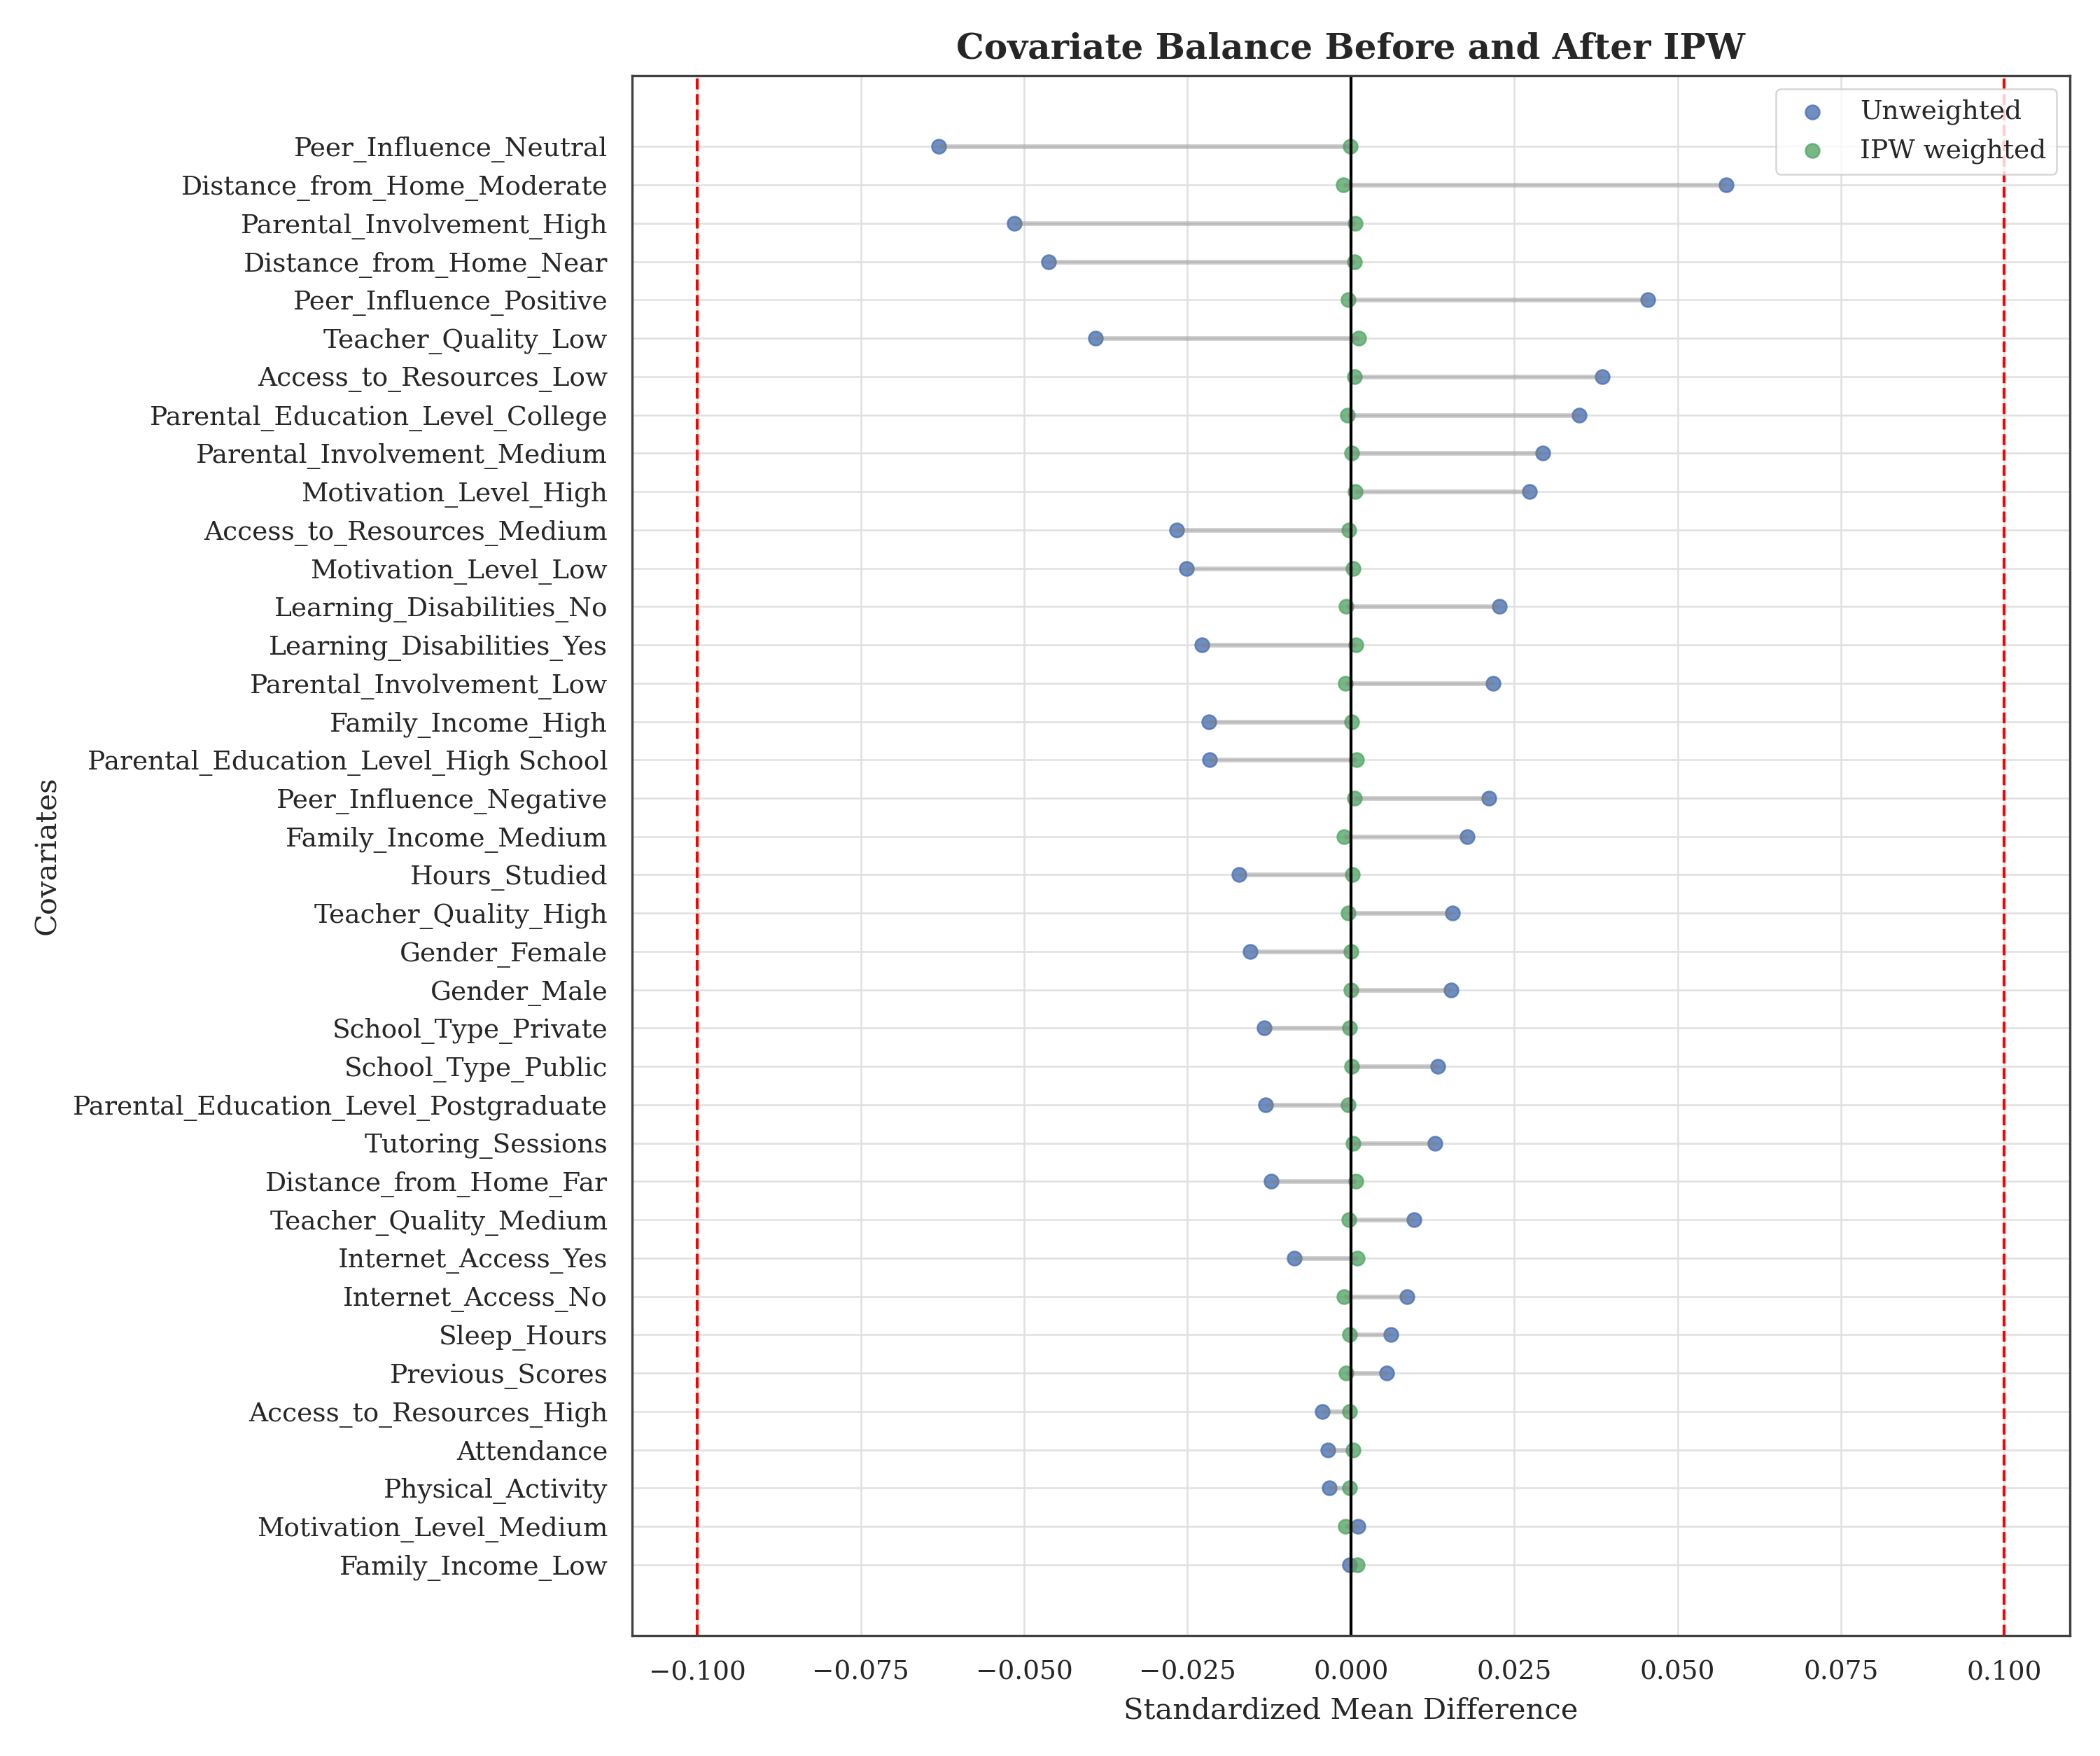
\includegraphics[width=\textwidth]{../figs/balance_ipw.png}
%         \caption{Covariate Balance Before and After IPW}
%         \label{fig:balance_ipw}
%     \end{subfigure}
%     \hfill
%     \begin{subfigure}{0.45\textwidth}
%         \centering
%         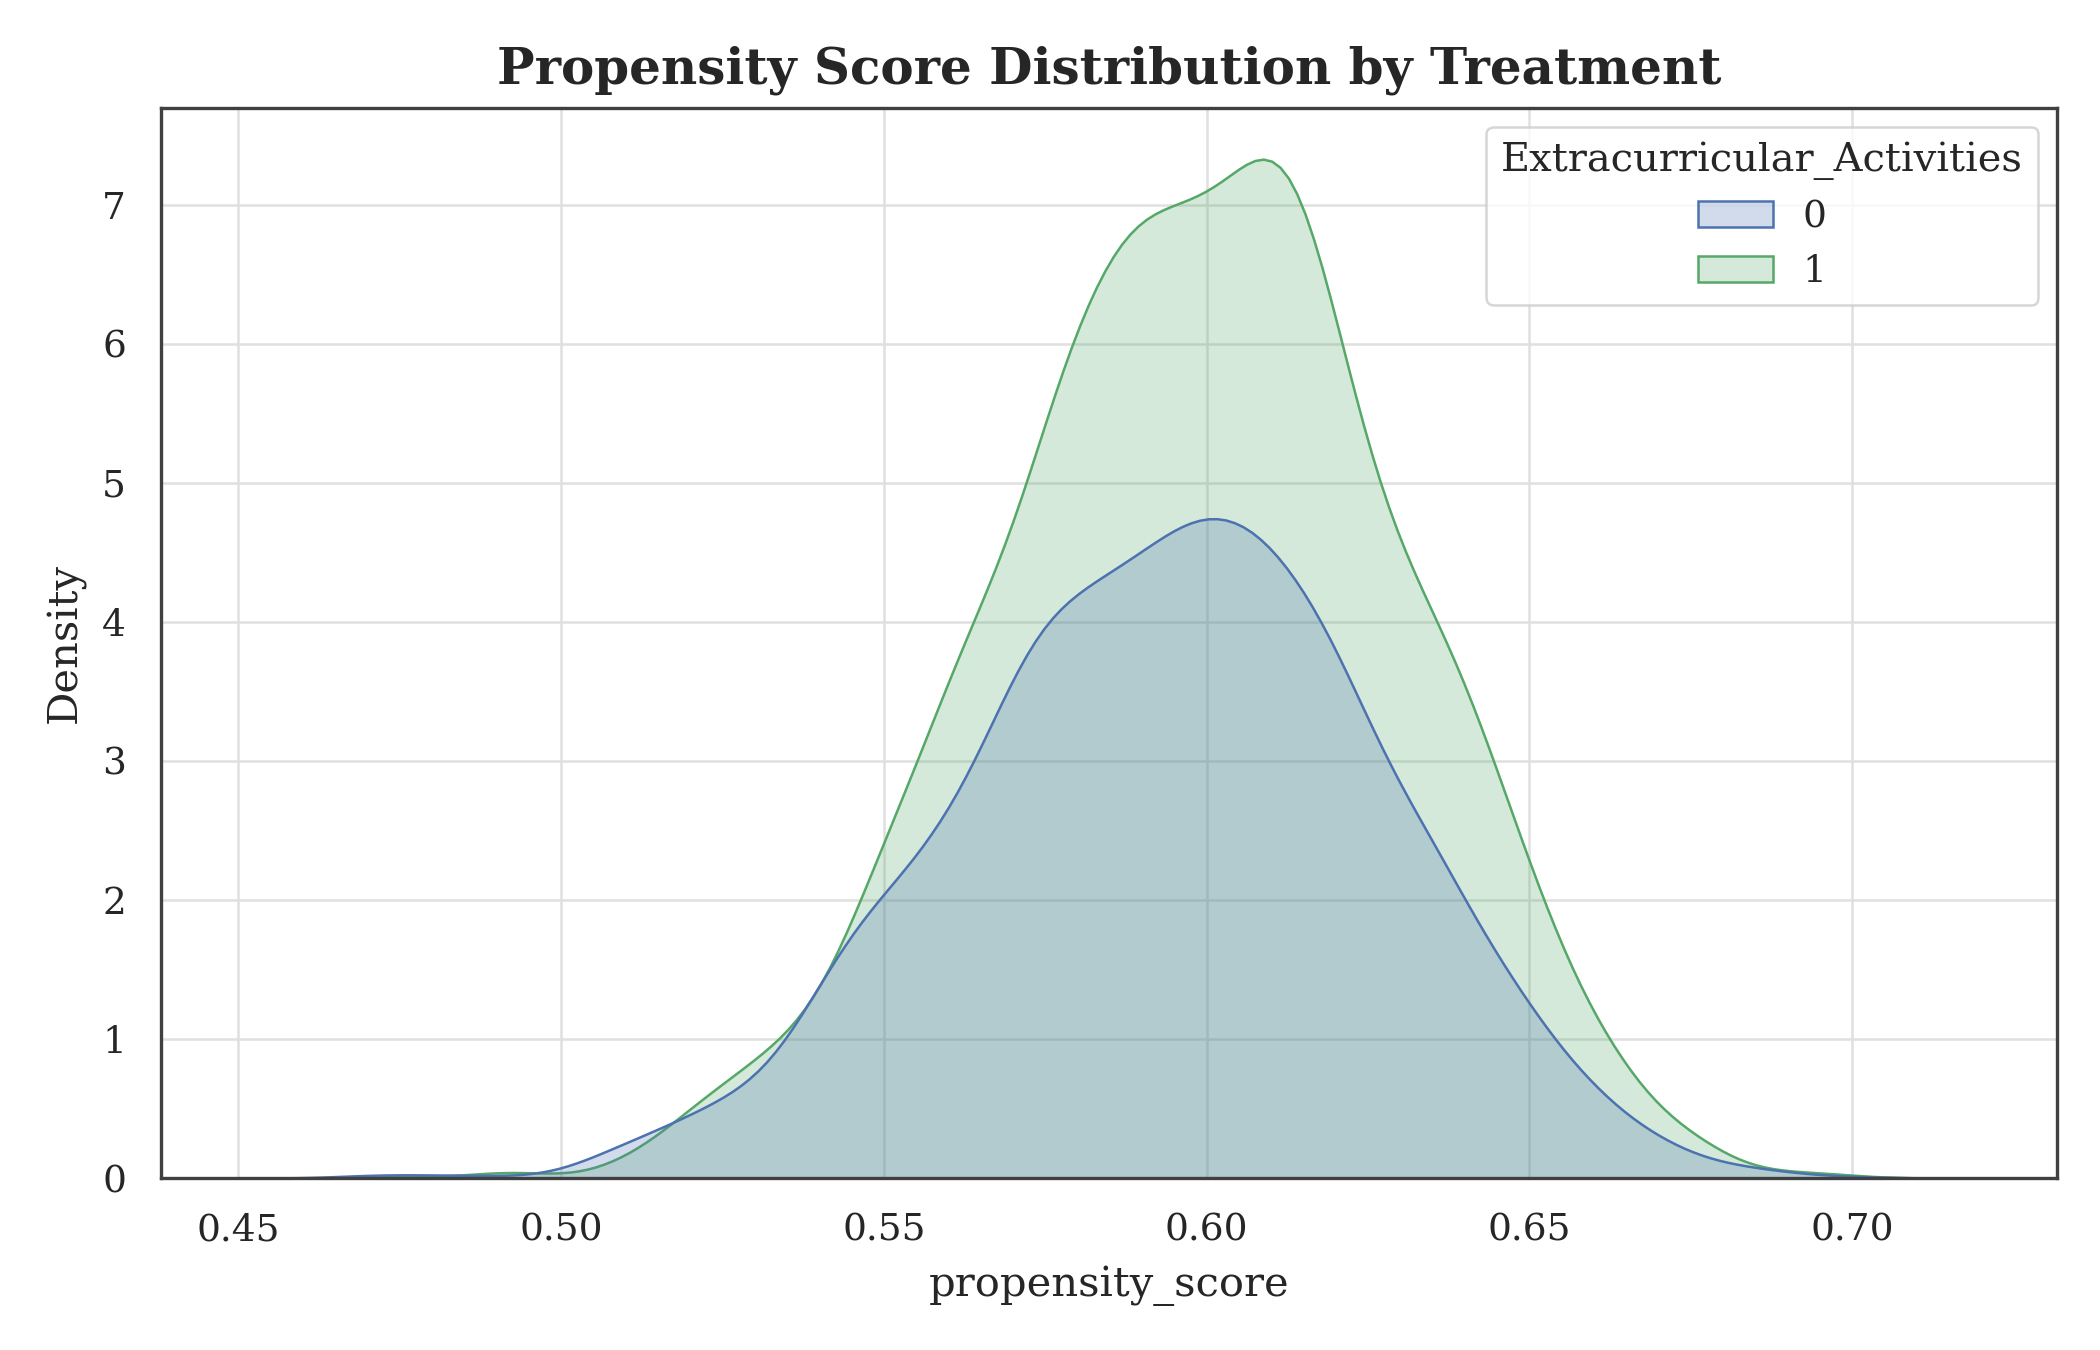
\includegraphics[width=\textwidth]{../figs/ps_distribution.png}
%         \caption{Distribution of Propensity Scores by Treatment Group}
%         \label{fig:ps_distribution}
%     \end{subfigure}

% \end{figure}

% The poor fit of the propensity score model gives us some confidence that the unconfoundedness assumption may hold, as the treatment assignment does not appear to be strongly driven by the observed covariates. The improved balance after weighting also supports the validity of the IPW approach for estimating the causal effect.

% \subsubsection{ATE Estimation}

% We apply the inverse probability weights to estimate the ATE using weighted least squares regression. The results are shown in Table~\ref{tab:ipw-results}. The estimated treatment effect is 0.562 (95\% CI: [0.462, 0.662], $p < 0.001$) when including all observations, which is consistent with the OLS estimate. After removing influential observations, the estimated effect decreases to 0.505 (95\% CI: [0.490, 0.521], $p < 0.001$), indicating that influential points have a noticeable impact on the magnitude of the estimated effect, although the positive association remains robust. 

% The 95\% confidence intervals in baseline outcome regression and IPW are quite similar, even the same after removing influential observations, which suggests that the IPW approach is providing a similar estimate of the treatment effect as the OLS model, lending credibility to the causal interpretation under the unconfoundedness assumption.

% \begin{table}[htbp]
% \centering
% \caption{Inverse Probability Weighted (IPW) Estimates with and without Influential Observations}
% \label{tab:ipw-results}
% \begin{tabular}{lccccc}
% \toprule
% Model & Effect & Std. Err. & 95\% CI & p-value & $N$ \\
% \midrule
% With influential observations 
% & 0.562 & 0.051 & [0.462, 0.662] & $<$0.001 & 6378 \\

% Without influential observations 
% & 0.505 & 0.008 & [0.490, 0.521] & $<$0.001 & 6323 \\

% \bottomrule
% \end{tabular}
% \end{table}


% \section{Key Findings and Interpretation}
% The results from both the OLS and IPW analyses consistently indicate a positive association between extracurricular activity participation and exam scores, with estimated effects around 0.5 to 0.6 points higher for students who participate in extracurricular activities compared to those who do not, after controlling for observed covariates. The robustness checks, including the removal of influential observations, show that while the magnitude of the estimated effect is sensitive to certain data points, the overall conclusion of a positive effect remains consistent. The exploration of treatment effect heterogeneity did not yield statistically significant interaction effects, suggesting that the benefit of extracurricular activities on exam scores does not vary strongly across different levels of motivation or study hours in this dataset. The propensity score diagnostics indicate that the IPW approach successfully balanced the covariates between treatment groups, lending credibility to the causal interpretation of the estimated effects under the unconfoundedness assumption.

% Based on these findings, we can cautiously conclude that participation in extracurricular activities is associated with improved academic performance as measured by exam scores. However, it is important to acknowledge the limitations of the analysis, including potential unobserved confounding and the observational nature of the data, which may affect the generalizability of the results.


\clearpage
\bibliographystyle{plain}
\bibliography{references}

\clearpage
\section*{Appendix}
\addcontentsline{toc}{section}{Appendix}
\appendix
\section{Data Summary Tables}\label{sec:data summary}

Here we present the summary statistics for both continuous and categorical variables in the original dataset. 
\begin{table}[htbp]
\centering
\caption{Summary Statistics for Continuous Variables}
\label{tab:continuous_summary}
\begin{tabular}{lrrrrrr}
\toprule
Variable & Mean & Std. Dev. & Min & Max & Null Count & Null Rate \\
\midrule
Hours\_Studied     & 19.98 & 5.99 & 1.00  & 44.00  & 0 & 0.000 \\
Attendance         & 79.98 & 11.55 & 60.00 & 100.00 & 0 & 0.000 \\
Sleep\_Hours       & 7.03  & 1.47 & 4.00  & 10.00  & 0 & 0.000 \\
Previous\_Scores   & 75.07 & 14.40 & 50.00 & 100.00 & 0 & 0.000 \\
Tutoring\_Sessions & 1.49  & 1.23 & 0.00  & 8.00   & 0 & 0.000 \\
Physical\_Activity & 2.97  & 1.03 & 0.00  & 6.00   & 0 & 0.000 \\
Exam\_Score        & 67.24 & 3.89 & 55.00 & 101.00 & 0 & 0.000 \\
\bottomrule
\end{tabular}
\end{table}

\begin{table}[H]
\centering
\caption{Summary Statistics for Categorical Variables}
\label{tab:categorical_summary}
\begin{tabularx}{\textwidth}{l c X l c c}
\toprule
Variable & No. of Categories  & Mode & Null Count & Null Rate \\
\midrule
Parental\_Involvement      & 3                     & Medium      & 0  & 0.000 \\
Access\_to\_Resources      & 3                   & Medium      & 0  & 0.000 \\
Extracurricular\_Activities& 2                            & Yes         & 0  & 0.000 \\
Motivation\_Level          & 3                    & Medium      & 0  & 0.000 \\
Internet\_Access           & 2                            & Yes         & 0  & 0.000 \\
Family\_Income             & 3                   & Low         & 0  & 0.000 \\
Teacher\_Quality           & 4                    & Medium      & 78 & 0.012 \\
School\_Type               & 2                      & Public      & 0  & 0.000 \\
Peer\_Influence            & 3          & Positive    & 0  & 0.000 \\
Learning\_Disabilities     & 2                             & No          & 0  & 0.000 \\
Parental\_Education\_Level & 4   & High School & 90 & 0.014 \\
Distance\_from\_Home       & 4                & Near        & 67 & 0.010 \\
Gender                     & 2                        & Male        & 0  & 0.000 \\
\bottomrule
\end{tabularx}
\end{table}


\section{Standardized Mean Differences for All Covariates}\label{sec: smd}

\begin{figure}[H]
\centering
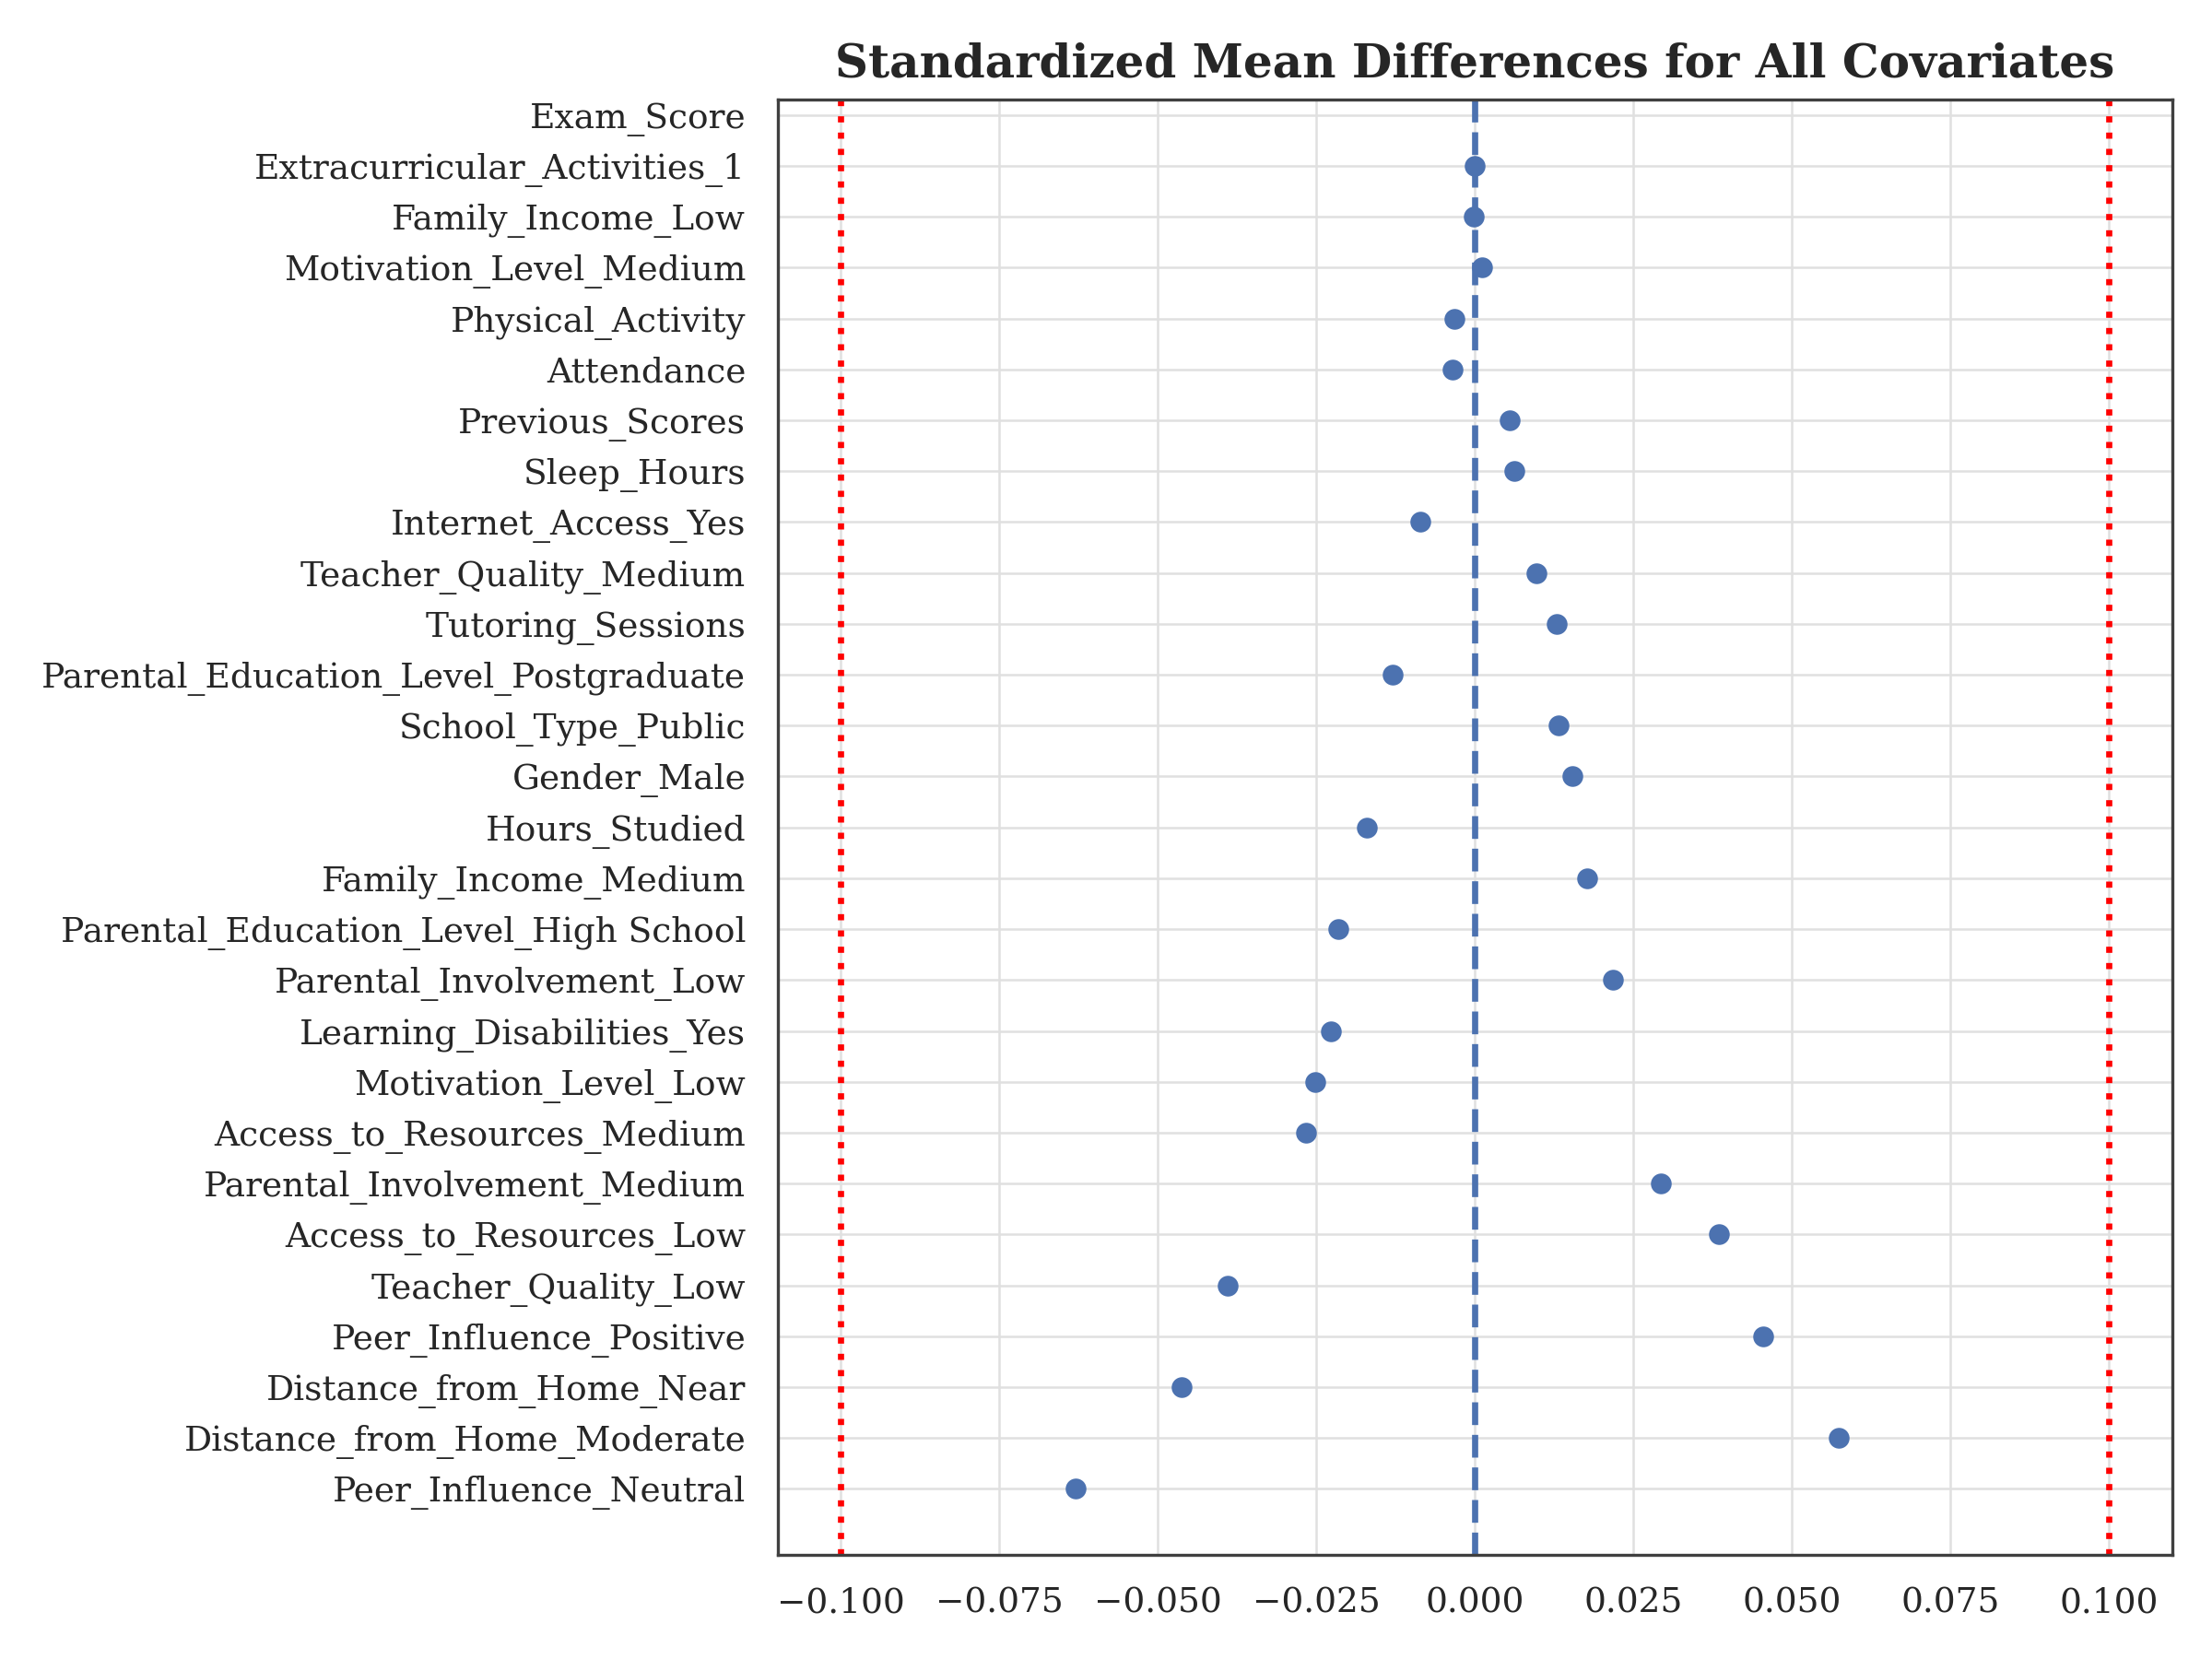
\includegraphics[width=0.8\textwidth]{../figs/smd_all.png}
\caption{Standardized Mean Differences for All Covariates}
\label{fig:smd_all}
\end{figure}



\section{Interaction Plots}\label{sec:interation-plot}

\begin{figure}[H]
\centering
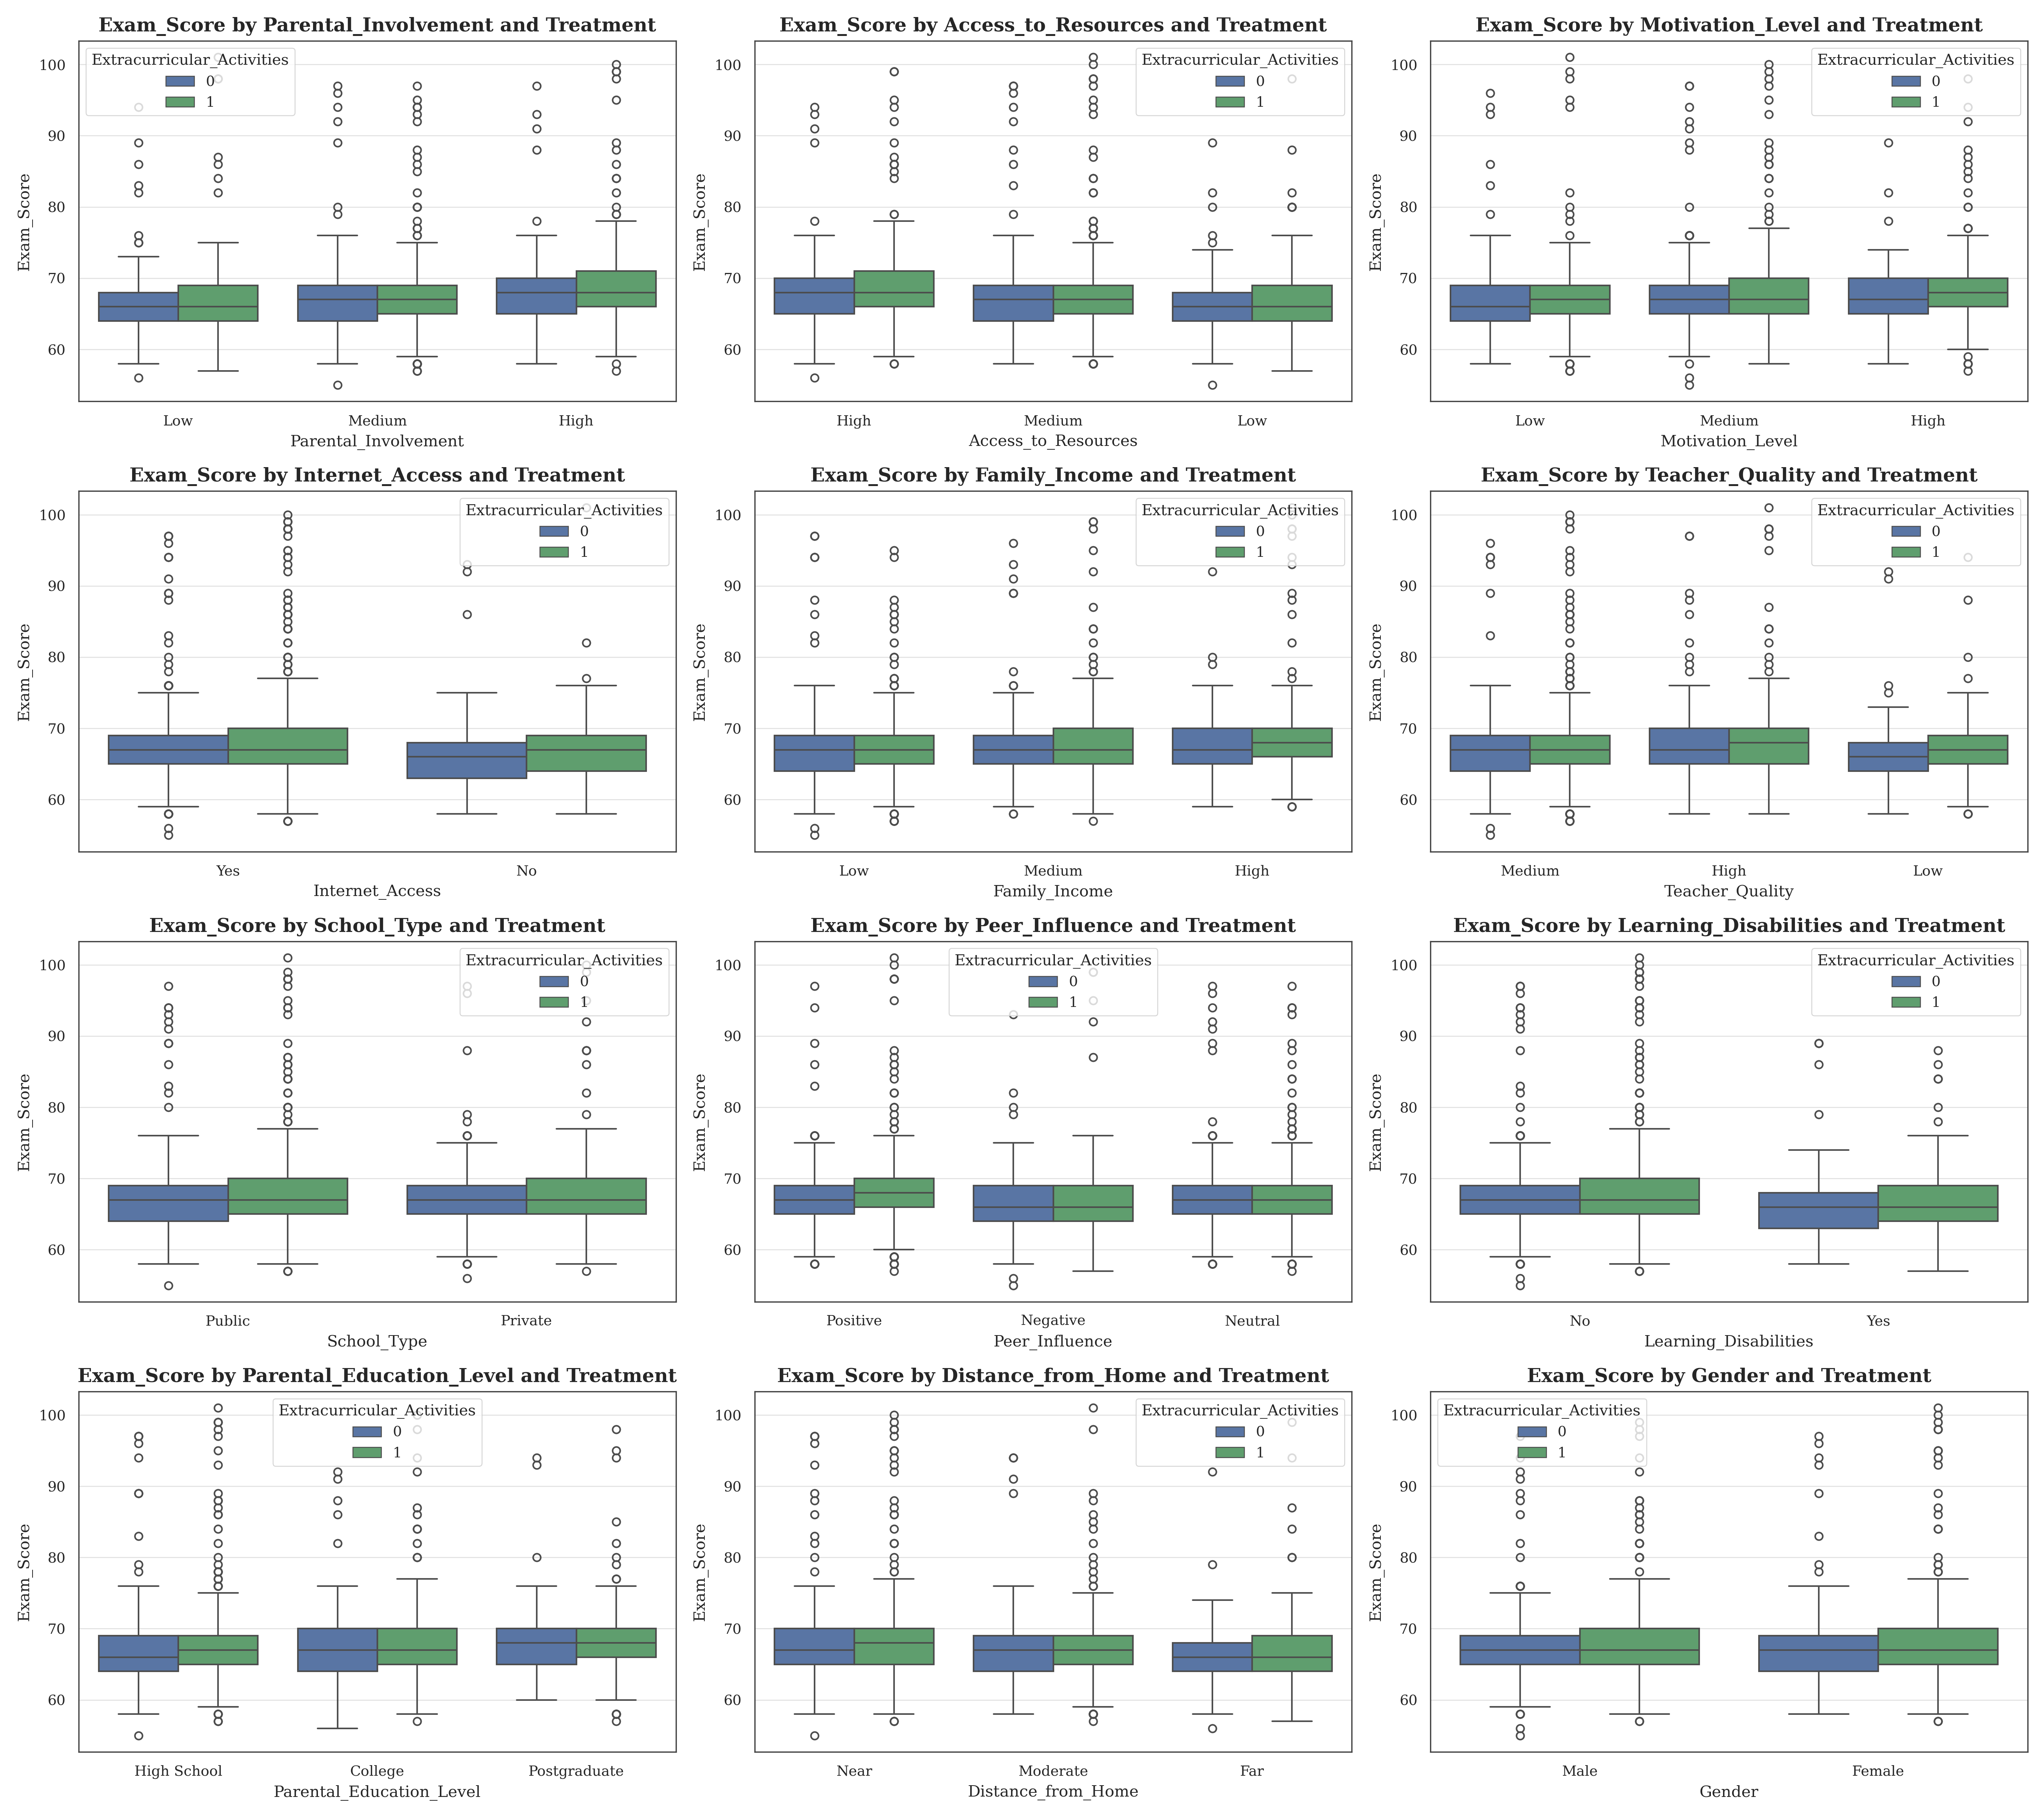
\includegraphics[width=1\textwidth]{../figs/cat_interactions.png}
\caption{Interaction effects between treatment and categorical covariates.}
\label{fig:cat_interactions}
\end{figure}  


\begin{figure}[H]
\centering
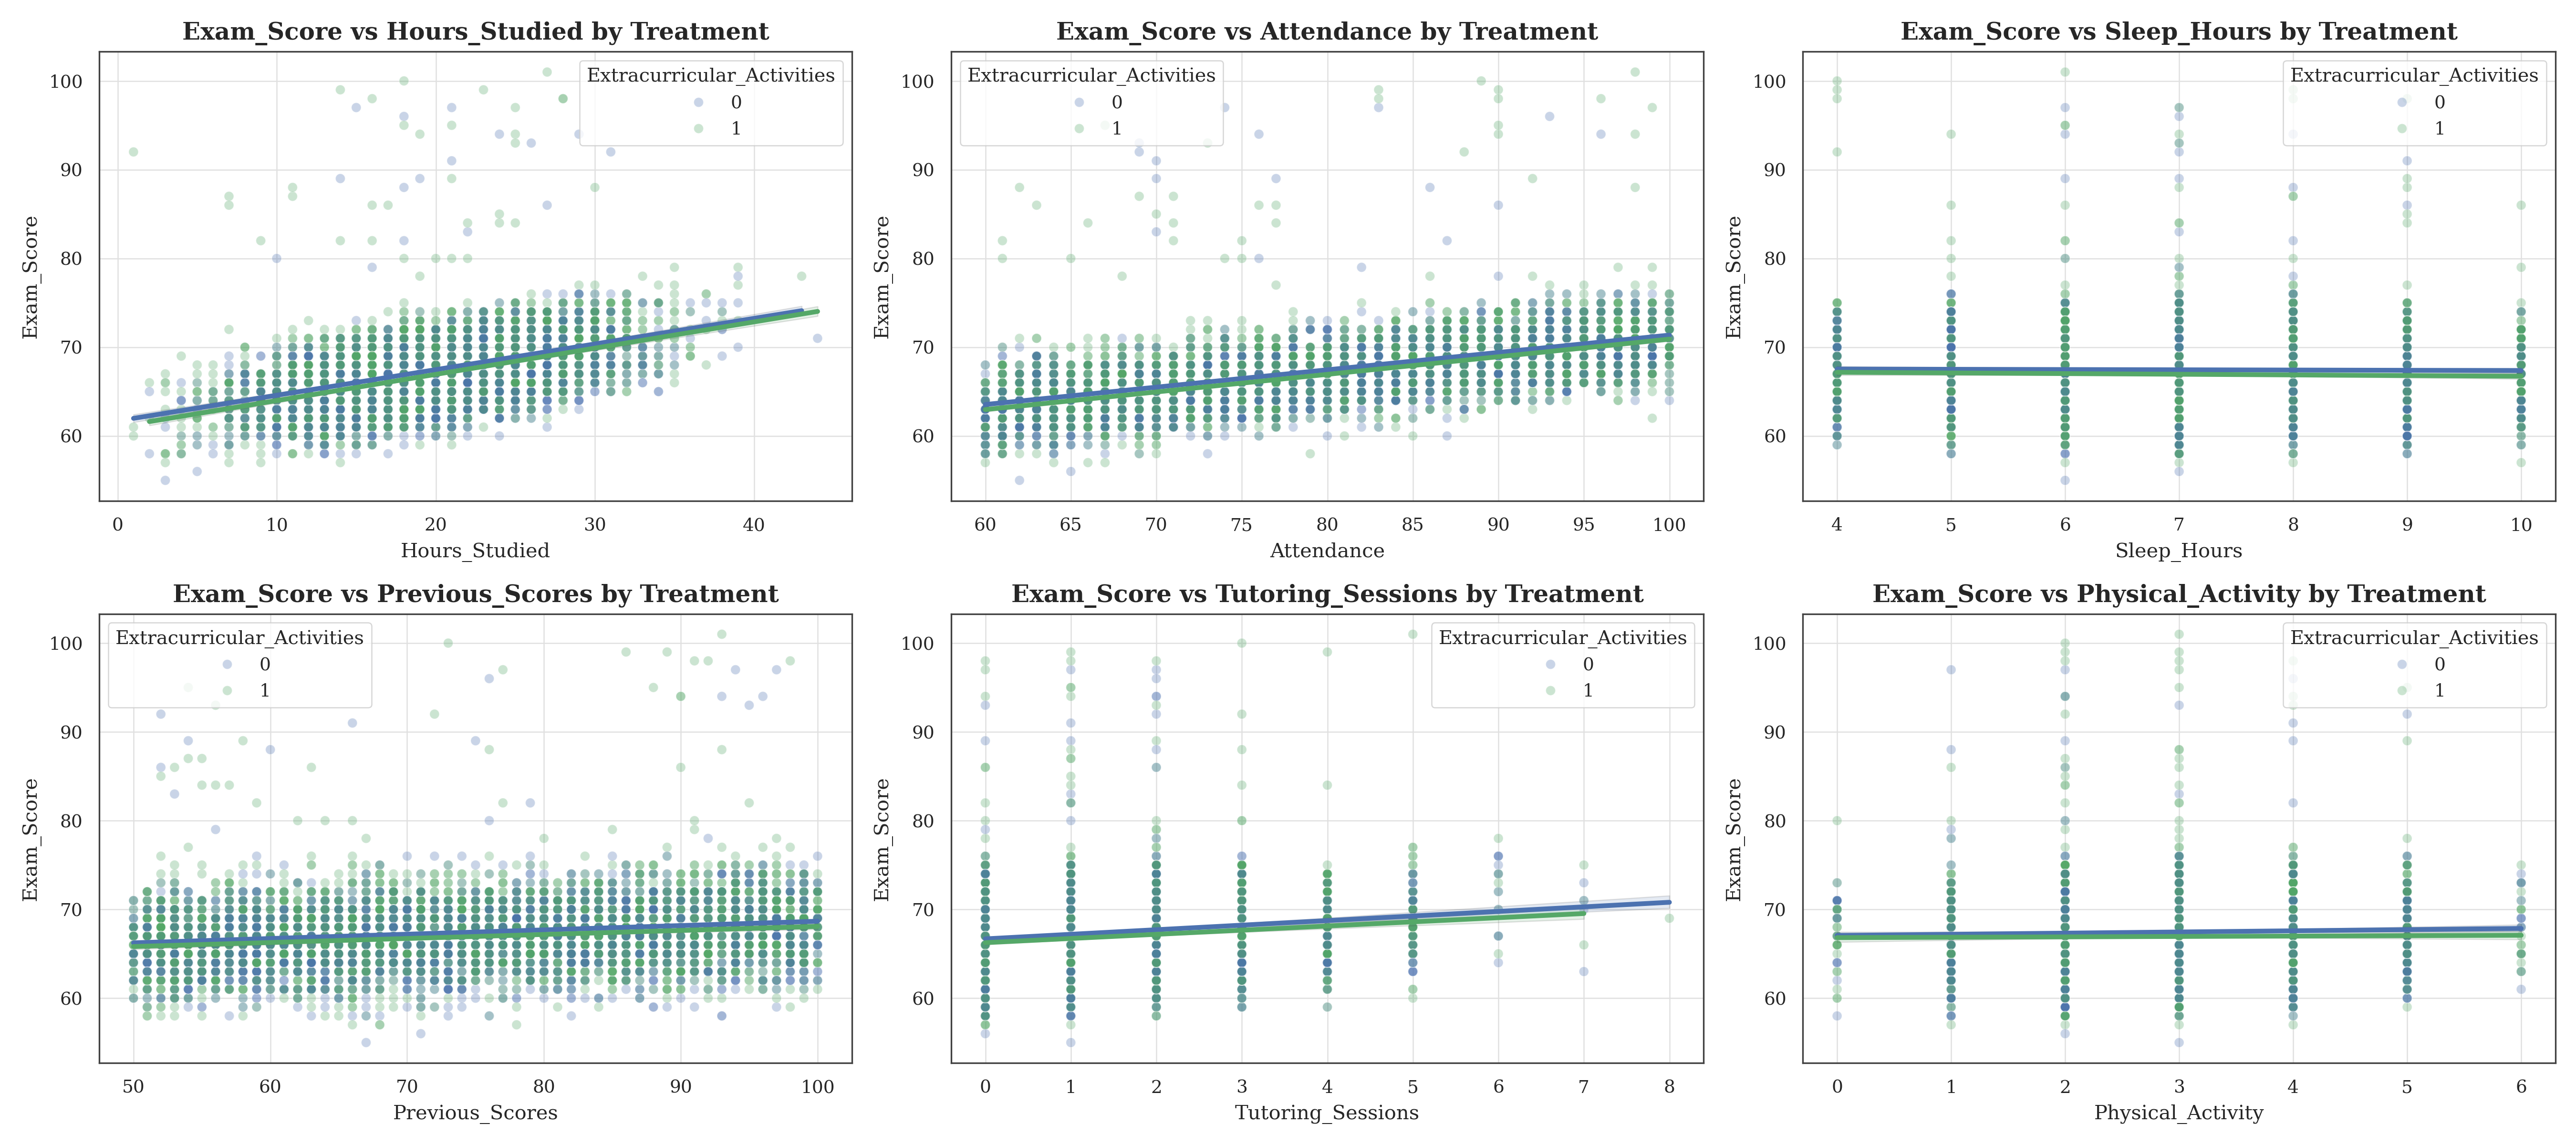
\includegraphics[width=1\textwidth]{../figs/num_interactions.png}
\caption{Interaction effects between treatment and continuous covariates.}
\label{fig:num_interactions}
\end{figure}





\end{document}
